\documentclass[11pt,a4paper]{article}

\usepackage[utf8]{inputenc}
\usepackage[T1]{fontenc}
\usepackage{lmodern}
\usepackage[margin=1in]{geometry}
\usepackage{amsmath,amssymb,amsfonts,bm}
\usepackage{booktabs}
\usepackage{graphicx}
\usepackage{float}
\usepackage{caption}
\usepackage{subcaption}
\usepackage{xcolor}
\usepackage{hyperref}
\usepackage{natbib}
\usepackage{microtype}

\definecolor{darkblue}{RGB}{20,60,120}
\hypersetup{
  colorlinks=true,
  linkcolor=darkblue,
  citecolor=darkblue,
  urlcolor=darkblue
}

\title{\textbf{Neuro-Symbolic Input-Skip Latent Binary Bayesian Neural Networks:\\ Differentiable Structural Learning, Rational Law Recovery, and Bayesian Logic Regression}}

\author{
  Aliaksandr Hubin\\
  \small Department of Mathematics, University of Oslo, Oslo, Norway\\
  \small Norwegian Computing Center, Oslo, Norway\\
  \small \texttt{aliaksah@math.uio.no}
}

\date{\today}

\begin{document}

\maketitle

\begin{abstract}
Discovering parsimonious, closed-form symbolic laws and interpretable Boolean interactions directly from noisy observational data while quantifying structural uncertainty remains a central challenge at the intersection of statistical machine learning and scientific discovery. Bayesian Generalized Nonlinear Models (BGNLMs) and Bayesian Logic Regression (BLR) formulate symbolic and logical structure discovery as Bayesian variable selection over recursively constructed nonlinear features, but rely on discrete transdimensional Markov chain Monte Carlo algorithms such as Genetically Modified Mode Jumping MCMC (GMJMCMC) that must traverse combinatorial tree spaces through sequential discrete mutations. Conversely, Latent Binary Bayesian Neural Networks (LBBNNs) with input-skip connections enable end-to-end differentiable structural learning via continuous variational inference over spike-and-slab edge indicators, yet standard piecewise-linear activations yield black-box subnetworks rather than closed-form algebraic expressions. In this work, we bridge these two paradigms by introducing Neuro-Symbolic Input-Skip LBBNNs. We replace homogeneous rectified linear units with a bank of domain-safe differentiable symbolic operators, continuous product-t-norm Boolean conjunction gates equipped with negated literal projections, and logarithmic-exponential composition pathways that parameterize multivariate power laws continuously in exponent space. To prevent deep compositional overfitting, we embed the BGNLM complexity prior directly into the spike-and-slab prior inclusion probabilities and introduce a symmetric bimodal Gaussian mixture slab prior that drives Boolean gate weights toward crisp literal assignments while keeping zero in a low-density valley. Because variational Kullback--Leibler regularization induces shrinkage bias on surviving continuous exponents, we formulate a two-stage inference protocol that freezes the variational Median Probability Model (MPM) active-path topology after structural learning, debiases surviving weights via unpenalized quasi-Newton and ordinary least squares refitting, and snaps continuous exponents to their simplest continued-fraction rationals under a Bayesian Information Criterion guard. Across four benchmark studies encompassing Bayesian logic regression, synthetic and real NASA exoplanet orbital mechanics, and the nonlinear Friedman benchmark, hierarchical linear mixed-effects evaluations against eight established statistical and symbolic regression baselines demonstrate that Neuro-Symbolic LBBNNs recover exact physical laws and parsimonious Boolean clauses while matching the oracle noise floor in out-of-sample generalization.
\end{abstract}

\noindent\textbf{Keywords:} Latent Binary Bayesian Neural Networks, Bayesian Generalized Nonlinear Models, Bayesian Logic Regression, Symbolic Regression, Spike-and-Slab Variational Inference, Mixed-Effects Evaluation

\section{Introduction}
\label{sec:intro}

A foundational tension in modern statistical modeling lies between the expressive flexibility of deep neural networks and the mechanistic interpretability of classical parsimonious regression. In the physical, biological, and epidemiological sciences, predictive accuracy alone is rarely sufficient; researchers seek compact mathematical expressions, such as algebraic power laws, trigonometric conservation identities, or Boolean risk rules, that extrapolate reliably beyond the training domain and admit domain-specific theoretical verification \citep{udrescu2020ai, cranmer2023interpretable, la2021contemporary}. Standard deep neural networks approximate such relationships through dense compositions of piecewise-linear or sigmoidal units. Even when post-hoc attribution measures are applied, the resulting representations remain distributed across hundreds of parameters and fail to extrapolate when covariates shift outside the convex hull of the training support \citep{rudin2019stop}.

Within the Bayesian paradigm, two distinct lines of work have addressed structural learning and parsimony from opposite directions. The first family comprises Bayesian Generalized Nonlinear Models (BGNLMs; \citealp{hubin2021bgnlm}) and Bayesian Logic Regression (BLR; \citealp{hubin2020bayesian}), as implemented in the \texttt{EMJMCMC} and \texttt{FBMS} packages \citep{frommlet2025fbms}. In BGNLMs, nonlinear scientific laws and higher-order Boolean conjunctions are represented as generalized linear predictors built from recursively composed univariate transformations, multiplicative interactions, and linear projections. Model uncertainty is quantified by placing complexity-penalized priors on the generated features and exploring the resulting transdimensional model space via Genetically Modified Mode Jumping Markov Chain Monte Carlo (GMJMCMC; \citealp{hubin2018mode, hubin2020adaptive}). Although GMJMCMC provides well-calibrated posterior inclusion probabilities across moderate feature spaces, its reliance on discrete evolutionary proposals creates a structural bottleneck whenever the true data-generating law requires a specific multi-step nested composition. For example, recovering Kepler's third law $a = M_*^{1/3} T^{2/3}$ in a discrete tree grammar requires sequentially proposing the quadratic transformation $T^2$, multiplying by stellar mass $M_* T^2$, and applying the cube-root operator $(M_* T^2)^{1/3}$ before simpler additive surrogates saturate the finite feature population.

The second family consists of Latent Binary Bayesian Neural Networks (LBBNNs; \citealp{hubin2024sparse, skaaret2024input, skaaret2026lbbnn}). LBBNNs place spike-and-slab priors directly on the synaptic weights $\bm{W}^{(l)} \circ \bm{\Gamma}^{(l)}$ of a deep neural network and perform scalable mean-field variational inference via the local reparameterization trick \citep{kingma2015variational} and continuous Concrete relaxations of the binary edge indicators \citep{maddison2016concrete}. Notably, the input-skip LBBNN architecture of \citet{skaaret2024input} concatenates the original input covariates $\bm{x}$ to the post-activation vector $\bm{u}^{(l-1)}$ at every hidden layer. This topological modification allows signals to bypass unnecessary intermediate layers, connects shallow linear terms directly to the output alongside deeper compositional pathways, and enables formal pruning of inactive edges via the Median Probability Model (MPM; \citealp{barbieri2004optimal}). However, because existing LBBNNs rely on homogeneous rectified linear, hyperbolic tangent, or silu activations, the pruned MPM subnetwork remains a piecewise-linear spline approximation rather than a closed-form symbolic equation.

Concurrently, differentiable symbolic regression networks such as Equation Learner (EQL) architectures \citep{martius2016extrapolation, sahoo2018learning, kim2020integration} have attempted to replace standard neural activations with elementary mathematical primitives ($\sin$, $\cos$, $\exp$, $\log$, and multiplication) trained under $\ell_1$ or smoothed $\ell_{0.5}$ penalties. While EQL demonstrates that backpropagation can guide structural search, purely frequentist penalty methods suffer from three acute pathologies: first, unprotected logarithmic, rational, and exponential units diverge or produce undefined gradients whenever pre-activations cross zero or grow large during stochastic optimization; second, uniform sparsity penalties lack depth- and complexity-aware Bayesian calibration, leading to nested compositions such as $\exp(\exp(x))$ when shallow linear terms suffice; and third, continuous shrinkage penalties bias the surviving parameter estimates toward zero, Perturbing fractional physical exponents such as $1/3 \approx 0.333$ into shrunken decimals such as $0.278$ that destroy exact symbolic law recovery.

In this paper, we resolve these limitations simultaneously by developing Neuro-Symbolic Input-Skip LBBNNs. Rather than searching over discrete expression trees via genetic mutations, we embed a heterogeneous bank of domain-safe symbolic primitives, differentiable product-t-norm Boolean logic gates, and logarithmic-exponential power-law pathways directly into the input-skip LBBNN architecture. We endow the binary structural indicators with BGNLM-inspired depth- and operator-complexity priors that penalize deep, non-smooth operators unless justified by the marginal likelihood. For Boolean logic gates, we replace the standard unimodal Gaussian slab prior with a symmetric bimodal Gaussian mixture slab centered at $\{-1, +1\}$ that actively repels active weights from zero and forces literal selection toward positive ($X_i$) or negated ($1 - X_i$) states. Finally, we decouple structural discovery from parameter estimation through a two-stage inference procedure: Stage 1 performs annealed variational inference with Kullback--Leibler (KL) warmup to isolate the MPM active-path topology, whereas Stage 2 freezes the binary MPM mask, eliminates shrinkage bias via unpenalized quasi-Newton (L-BFGS) and ordinary least squares (OLS) refitting, and snaps continuous exponents to parsimonious continued-fraction rationals under a Bayesian Information Criterion (BIC) guard.

The remainder of the article is organized as follows. Section~\ref{sec:methods} presents the mathematical formulation of the Neuro-Symbolic Input-Skip LBBNN, the domain-safe operator library, the hierarchical prior specification, and the two-stage inference and symbolic extraction algorithms. Section~\ref{sec:experiments} details the four simulation and empirical benchmark studies, comparing our framework against eight established statistical, machine learning, and symbolic regression baselines through hierarchical linear mixed-effects models. Section~\ref{sec:discussion} synthesizes our empirical findings, discusses methodological limitations and avenues for future research, and concludes the paper.

\section{Methodology}
\label{sec:methods}

\subsection{Input-skip latent binary Bayesian neural networks}
\label{sec:methods:arch}

Consider a supervised learning problem with $n$ observations $\mathcal{D} = \{(\bm{x}_m, y_m)\}_{m=1}^n$, where $\bm{x}_m = (x_{m1}, \dots, x_{mp})^\top \in \mathbb{R}^p$ denotes a $p$-dimensional vector of covariates and $y_m \in \mathbb{R}$ is the response variable. An $L$-layer Input-Skip LBBNN \citep{skaaret2024input, skaaret2026lbbnn} defines a hierarchical composition over hidden layer post-activation vectors $\bm{u}^{(l)} = (u_1^{(l)}, \dots, u_{n^{(l)}}^{(l)})^\top \in \mathbb{R}^{n^{(l)}}$ for $l = 1, \dots, L-1$, culminating in a linear readout layer $l = L$ with $n^{(L)} = 1$. To enable adaptive compositional depth, we set $\tilde{\bm{u}}^{(0)} = \bm{x} \in \mathbb{R}^p$ for the first hidden layer ($d_{\text{in}}^{(1)} = p$), and for every subsequent layer $l = 2, \dots, L$, we concatenate the raw input vector $\bm{x}$ directly to the previous hidden layer's post-activations:
\begin{equation}
\label{eq:input_skip_concat}
\tilde{\bm{u}}^{(l-1)} = \begin{bmatrix} \bm{u}^{(l-1)} \\ \bm{x} \end{bmatrix} = \left[u_1^{(l-1)}, \dots, u_{n^{(l-1)}}^{(l-1)}, x_1, \dots, x_p\right]^\top \in \mathbb{R}^{d_{\text{in}}^{(l)}}, \qquad d_{\text{in}}^{(l)} = n^{(l-1)} + p.
\end{equation}

In contrast to standard LBBNNs where all hidden neurons share a single homogeneous activation function, each hidden layer $l \in \{1, \dots, L-1\}$ in a Neuro-Symbolic LBBNN partitions its $n^{(l)}$ neurons across an ordered bank of heterogeneous mathematical operators $\bm{\sigma}^{(l)} = (\sigma_1^{(l)}, \dots, \sigma_{n^{(l)}}^{(l)})^\top$. Let $\bm{W}^{(l)} = (w_{ji}^{(l)}) \in \mathbb{R}^{n^{(l)} \times d_{\text{in}}^{(l)}}$ denote the continuous synaptic weight matrix of layer $l$, $\bm{\Gamma}^{(l)} = (\gamma_{ji}^{(l)}) \in \{0, 1\}^{n^{(l)} \times d_{\text{in}}^{(l)}}$ denote the corresponding matrix of latent binary inclusion indicators, and $\bm{b}^{(l)} = (b_1^{(l)}, \dots, b_{n^{(l)}}^{(l)})^\top \in \mathbb{R}^{n^{(l)}}$ denote the neuron bias vector. For layers $l = 1, \dots, L-1$, the pre-activation $z_j^{(l)}$ and post-activation $u_j^{(l)}$ of neuron $j \in \{1, \dots, n^{(l)}\}$ are given by
\begin{equation}
\label{eq:layer_forward}
z_j^{(l)} = \sum_{i=1}^{d_{\text{in}}^{(l)}} \gamma_{ji}^{(l)} w_{ji}^{(l)} \tilde{u}_i^{(l-1)} + b_j^{(l)}, \qquad u_j^{(l)} = \sigma_j^{(l)}\!\left(z_j^{(l)}\right),
\end{equation}
and the output layer $l = L$ forms a sparse linear combination of all top-level hidden features and direct input-skip covariates:
\begin{equation}
\label{eq:output_readout}
\hat{y}(\bm{x}) = u_1^{(L)} = b_1^{(L)} + \sum_{i=1}^{d_{\text{in}}^{(L)}} \gamma_{1i}^{(L)} w_{1i}^{(L)} \tilde{u}_i^{(L-1)}.
\end{equation}
When all binary indicators are fixed to their deterministic MPM states $\hat{\gamma}_{ji}^{(l)} \in \{0, 1\}$, Equation~\eqref{eq:output_readout} expands algebraically into a BGNLM additive predictor $\hat{y}(\bm{x}) = \beta_0 + \sum_{k \in \mathcal{A}} \beta_k f_k(\bm{x})$, where the active basis functions $f_k(\bm{x})$ correspond to the surviving directed paths through the operator graph.

\subsection{Differentiable symbolic and Boolean operator library}
\label{sec:methods:operators}

Arbitrary compositions of elementary mathematical functions quickly encounter domain violations during stochastic gradient descent whenever pre-activations $z_j^{(l)}$ cross zero or diverge in magnitude. We design a domain-safe, continuously differentiable operator library $\mathcal{G}$ stabilized by a small numerical constant $\varepsilon = 10^{-4}$. For algebraic and transcendental regression, $\mathcal{G}$ includes the identity map $\sigma_{\text{id}}(z) = z$, polynomial powers $\sigma_{\text{sq}}(z) = z^2$ and $\sigma_{\text{cb}}(z) = z^3$, periodic primitives $\sigma_{\sin}(z) = \sin(z)$ and $\sigma_{\cos}(z) = \cos(z)$, the stabilized reciprocal $\sigma_{\text{inv}}(z) = z / (z^2 + \varepsilon)$, the stabilized square root $\sigma_{\text{sqrt}}(z) = \sqrt{|z| + \varepsilon}$, the magnitude logarithm $\sigma_{\log}(z) = \log(|z| + \varepsilon)$, and the upper-clamped exponential $\sigma_{\exp}(z) = \exp(\min(z, 10))$.

To discover exact multivariate monomials and fractional power laws of the form $f(\bm{x}) = c \prod_{i \in S} x_i^{w_i}$ without resorting to discrete combinatorics over rational root primitives, we introduce a dedicated parameter-free input logarithm neuron $\sigma_{\text{clog}}$. In Layer $l=1$, the $j$-th $\sigma_{\text{clog}}$ neuron is wired one-to-one to the $j$-th positive input covariate $x_j$ with unit weight and zero bias, computing $u_j^{(1)} = \log(\max(x_j, \varepsilon))$. When an exponential neuron $\sigma_{\exp}$ in Layer $l=2$ connects to the $\sigma_{\text{clog}}$ block of Layer $1$, its post-activation evaluates to
\begin{equation}
\label{eq:clog_exp_pathway}
u_r^{(2)} = \exp\!\left(b_r^{(2)} + \sum_{j=1}^p \gamma_{rj}^{(2)} w_{rj}^{(2)} \log(x_j)\right) = e^{b_r^{(2)}} \prod_{j : \gamma_{rj}^{(2)} = 1} x_j^{w_{rj}^{(2)}}.
\end{equation}
Consequently, the discrete structural indicator $\gamma_{rj}^{(2)} \in \{0, 1\}$ determines whether covariate $x_j$ participates in the $r$-th multiplicative law, while the continuous synaptic weight $w_{rj}^{(2)} \in \mathbb{R}$ directly parameterizes its real exponent! This transforms the combinatorial tree search for nested fractional powers into smooth gradient optimization in log-exponent space.

To unify continuous symbolic discovery with Bayesian Logic Regression \citep{ruczinski2003logic, hubin2020bayesian} over binary covariates $\tilde{u}_i^{(l-1)} \in [0, 1]$, we introduce differentiable product-t-norm conjunction ($\sigma_{\text{and}}$) and probabilistic-sum disjunction ($\sigma_{\text{or}}$) neurons. Unlike univariate activations applied to a linear sum $z_j^{(l)}$, a logic neuron operates directly on the matrix of incoming connections by mapping each weight-indicator pair $(\gamma_{ji}^{(l)}, w_{ji}^{(l)})$ to a smooth literal inclusion gate $s_{ji}^{(l)} \in [0, 1]$ and a literal polarity projection $\ell_{ji}^{(l)}(\tilde{u}_i^{(l-1)}) \in [0, 1]$:
\begin{equation}
\label{eq:literal_projection}
\begin{aligned}
s_{ji}^{(l)} &= \gamma_{ji}^{(l)} \tanh\!\left(\left|w_{ji}^{(l)}\right|\right), \\
\ell_{ji}^{(l)}\!\left(\tilde{u}_i^{(l-1)}\right) &= \frac{1 + \tanh\!\left(\kappa w_{ji}^{(l)}\right)}{2}\,\tilde{u}_i^{(l-1)} + \frac{1 - \tanh\!\left(\kappa w_{ji}^{(l)}\right)}{2}\!\left(1 - \tilde{u}_i^{(l-1)}\right),
\end{aligned}
\end{equation}
where $\kappa = 5.0$ controls the sharpness of the polarity transition. Using the Gödel--product t-norm relaxation, the conjunction neuron $\sigma_{\text{and}}$ and disjunction neuron $\sigma_{\text{or}}$ compute
\begin{equation}
\label{eq:logic_neurons}
u_{j,\text{and}}^{(l)} = \prod_{i=1}^{d_{\text{in}}^{(l)}} \left[1 - s_{ji}^{(l)}\!\left(1 - \ell_{ji}^{(l)}(\tilde{u}_i^{(l-1)})\right)\right], \qquad u_{j,\text{or}}^{(l)} = 1 - \prod_{i=1}^{d_{\text{in}}^{(l)}} \left[1 - s_{ji}^{(l)} \ell_{ji}^{(l)}(\tilde{u}_i^{(l-1)})\right].
\end{equation}
Inspection of Equations~\eqref{eq:literal_projection}--\eqref{eq:logic_neurons} reveals three exact boundary properties. First, when an edge is pruned ($\gamma_{ji}^{(l)} = 0$), its gate vanishes ($s_{ji}^{(l)} = 0$), rendering the $i$-th multiplicative factor identically equal to $1$ in $u_{j,\text{and}}^{(l)}$ and $0$ in $u_{j,\text{or}}^{(l)}$ so that inactive inputs have zero influence on the clause. Second, when $\gamma_{ji}^{(l)} = 1$ and $w_{ji}^{(l)} \approx +1$, $\ell_{ji}^{(l)}(\tilde{u}_i^{(l-1)}) \to \tilde{u}_i^{(l-1)}$, encoding the positive literal $X_i$. Third, when $\gamma_{ji}^{(l)} = 1$ and $w_{ji}^{(l)} \approx -1$, $\ell_{ji}^{(l)}(\tilde{u}_i^{(l-1)}) \to 1 - \tilde{u}_i^{(l-1)}$, encoding the negated literal $\neg X_i$ without requiring separate negation layers.

\subsection{Complexity-penalized and bimodal spike-and-slab priors}
\label{sec:methods:priors}

In BGNLM \citep{hubin2021bgnlm}, the prior inclusion probability of a generated feature $f_j(\bm{x})$ decreases exponentially with its operational complexity to enforce Occam's razor. We translate this principle directly to the network topology by assigning each operator $\sigma \in \mathcal{G}$ an intrinsic complexity cost $c(\sigma) \ge 0$: specifically, $c(\sigma_{\text{id}}) = 0.5$, $c(\sigma_{\text{clog}}) = c(\sigma_{\text{sq}}) = c(\sigma_{\text{cb}}) = c(\sigma_{\text{and}}) = c(\sigma_{\text{or}}) = 1.0$, $c(\sigma_{\log}) = c(\sigma_{\exp}) = c(\sigma_{\sin}) = c(\sigma_{\cos}) = c(\sigma_{\text{sqrt}}) = 1.5$, and $c(\sigma_{\text{inv}}) = 2.0$. Each binary indicator $\gamma_{ji}^{(l)} \sim \mathrm{Bernoulli}(\pi_{ji}^{(l)})$ is assigned a layer- and neuron-specific prior inclusion probability $\pi_{ji}^{(l)}$ governed by
\begin{equation}
\label{eq:symbolic_prior}
\pi_{ji}^{(l)} = \frac{1}{1 + \exp\!\left(\operatorname{logit}(1 - \pi_0) + \beta_{\text{depth}}(l - 1) + \beta_{\text{comp}}\,c(\sigma_j^{(l)})\right)},
\end{equation}
where $\pi_0 \in (0, 1)$ is the baseline inclusion probability, $\beta_{\text{depth}} \ge 0$ penalizes compositional depth, and $\beta_{\text{comp}} \ge 0$ penalizes operator complexity. For connections feeding into the linear readout layer $l = L$ directly from the input-skip block, $c(\sigma)$ is set to $0$, ensuring that direct linear main effects experience the highest prior inclusion probability in the network.

Conditional on $\gamma_{ji}^{(l)}$, the synaptic weight $w_{ji}^{(l)}$ follows a spike-and-slab prior $p(w_{ji}^{(l)} \mid \gamma_{ji}^{(l)}) = \gamma_{ji}^{(l)} p_{\text{slab}}(w_{ji}^{(l)}) + (1 - \gamma_{ji}^{(l)})\delta_0(w_{ji}^{(l)})$, where $\delta_0$ is the Dirac point mass at zero. For continuous algebraic and transcendental neurons, we employ the standard zero-mean Gaussian slab $p_{\text{slab}}(w) = \mathcal{N}(w; 0, \sigma_w^{2(l)})$. For Boolean logic gates ($\sigma_j^{(l)} \in \{\sigma_{\text{and}}, \sigma_{\text{or}}\}$), however, a zero-mean Gaussian slab places maximum prior density at $w = 0$, which shrinks active literal gates $s_{ji}^{(l)} = \tanh(|w_{ji}^{(l)}|)$ toward zero and blurs the polarity sign in Equation~\eqref{eq:literal_projection}. We therefore introduce a symmetric bimodal Gaussian mixture slab prior for all logic gate rows:
\begin{equation}
\label{eq:bimodal_slab}
p_{\text{logic-slab}}\!\left(w_{ji}^{(l)}\right) = \frac{1}{2}\,\mathcal{N}\!\left(w_{ji}^{(l)}; +1, \sigma_L^2\right) + \frac{1}{2}\,\mathcal{N}\!\left(w_{ji}^{(l)}; -1, \sigma_L^2\right), \qquad \sigma_L = 0.28.
\end{equation}
As illustrated in Figure~\ref{fig:priors_dynamics}(c), Equation~\eqref{eq:bimodal_slab} places $w = 0$ in a deep low-density trough while creating symmetric potential wells at $w = +1$ (positive literal $X_i$) and $w = -1$ (negated literal $\neg X_i$). Under a Gaussian variational slab $q(w_{ji}^{(l)} \mid \gamma_{ji}^{(l)} = 1) = \mathcal{N}(\mu_{ji}^{(l)}, s_{ji}^{2(l)})$ with posterior inclusion probability $\alpha_{ji}^{(l)} = (1 + \exp(-\lambda_{ji}^{(l)}))^{-1}$, the exact KL divergence decomposes analytically except for the smooth bimodal slab expectation, for which we employ the tight log-sum-exp upper bound
\begin{equation}
\label{eq:kl_bimodal}
\begin{aligned}
\mathrm{KL}_{\text{logic}}\!\left(\mu_{ji}^{(l)}, s_{ji}^{(l)}, \alpha_{ji}^{(l)}\right) &= \alpha_{ji}^{(l)}\!\left[\frac{1}{2}\log\!\left(\frac{\sigma_L^2}{s_{ji}^{2(l)}}\right) - \frac{1}{2} + \frac{s_{ji}^{2(l)} + (\mu_{ji}^{(l)})^2 + 1}{2\sigma_L^2} - \log\cosh\!\left(\frac{\mu_{ji}^{(l)}}{\sigma_L^2}\right)\right] \\
&\quad + \mathrm{KL}_{\text{Bern}}\!\left(\alpha_{ji}^{(l)} \,\|\, \pi_{ji}^{(l)}\right),
\end{aligned}
\end{equation}
where $\mathrm{KL}_{\text{Bern}}(\alpha \,\|\, \pi) = \alpha \log(\alpha / \pi) + (1 - \alpha)\log((1 - \alpha)/(1 - \pi))$.

\begin{figure}[t!]
  \centering
  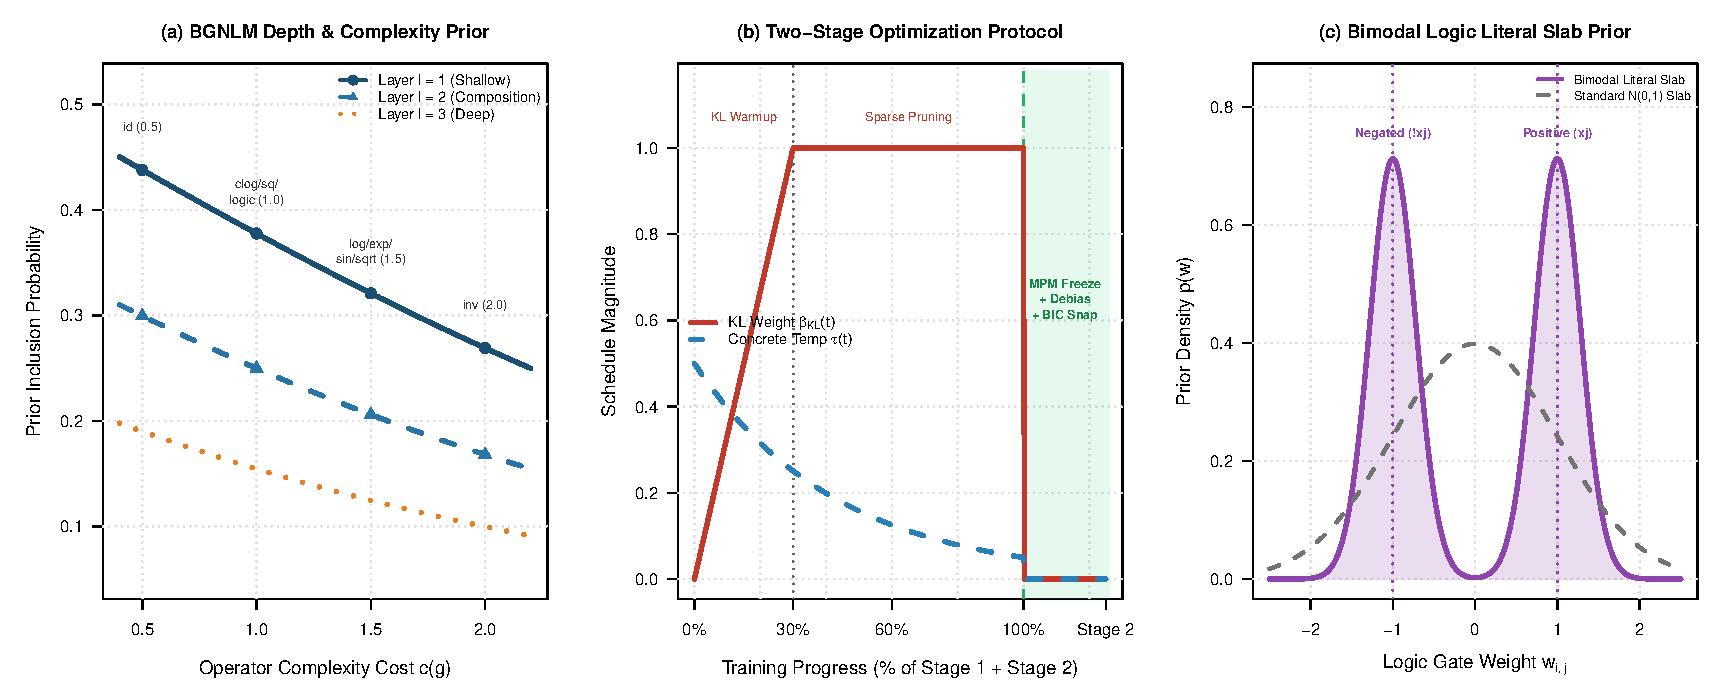
\includegraphics[width=\textwidth]{figures/fig1_priors_and_dynamics.pdf}
  \caption{Mathematical components of the Neuro-Symbolic Input-Skip LBBNN. (a) Prior inclusion probability $\pi_{ji}^{(l)}$ as a function of operator complexity cost $c(\sigma)$ across network depths $l \in \{1, 2, 3\}$ under Equation~\eqref{eq:symbolic_prior}. (b) Two-stage optimization schedules showing linear KL warmup $\beta_{\text{KL}}(t)$ and exponential Concrete temperature decay $\tau(t)$ during Stage 1 structural learning, followed by the Stage 2 MPM topological freeze, weight debiasing, and BIC rational snapping phase. (c) Symmetric bimodal Gaussian mixture slab prior $p_{\text{logic-slab}}(w)$ centered at $w = \pm 1$ compared against a standard $\mathcal{N}(0, 1)$ slab.}
  \label{fig:priors_dynamics}
\end{figure}

\subsection{Two-stage variational structural learning, debiasing, and rational snapping}
\label{sec:methods:training}

Given the variational posterior $q_{\bm{\eta}}(\bm{W}, \bm{\Gamma})$ parameterized by $\bm{\eta} = \{\mu_{ji}^{(l)}, \rho_{ji}^{(l)}, \lambda_{ji}^{(l)}\}$ with $s_{ji}^{(l)} = \log(1 + \exp(\rho_{ji}^{(l)}))$, Stage 1 maximizes the annealed Evidence Lower Bound (ELBO) over $T_1$ epochs:
\begin{equation}
\label{eq:annealed_elbo}
\begin{aligned}
\mathcal{L}_{\text{Stage 1}}(\bm{\eta}; t) &= -\mathbb{E}_{q_{\bm{\eta}}(\bm{W}, \bm{\Gamma}; \tau(t))}\!\left[\log p(\bm{y} \mid \bm{X}, \bm{W}, \bm{\Gamma})\right] \\
&\quad + \beta_{\text{KL}}(t) \sum_{l=1}^L \sum_{j=1}^{n^{(l)}} \sum_{i=1}^{d_{\text{in}}^{(l)}} \mathrm{KL}\!\left(q(w_{ji}^{(l)}, \gamma_{ji}^{(l)}) \,\|\, p(w_{ji}^{(l)}, \gamma_{ji}^{(l)})\right).
\end{aligned}
\end{equation}
As shown in Figure~\ref{fig:priors_dynamics}(b), the KL weight follows a linear warmup schedule $\beta_{\text{KL}}(t) = \min(1, t / T_{\text{warmup}})$ with $T_{\text{warmup}} = 0.30\,T_1$ so that candidate symbolic pathways can align with the data signal before the sparsity prior prunes low-utility connections, while the Concrete relaxation temperature decays exponentially via $\tau(t) = \tau_{\text{init}}(\tau_{\text{final}} / \tau_{\text{init}})^{t / T_1}$ from $\tau_{\text{init}} = 0.50$ to $\tau_{\text{final}} = 0.05$.

At the conclusion of Stage 1, we compute the MPM active-path indicators $\hat{\gamma}_{ji}^{\text{path}(l)} = \mathbb{I}(\alpha_{ji}^{\text{path}(l)} > 0.5)$ by propagating path connectivity backward from the output layer $l = L$ to $l = 1$ \citep{skaaret2024input}, eliminating dangling edges that do not reach $\hat{y}(\bm{x})$. Although Stage 1 reliably isolates the sparse MPM graph topology, the surviving posterior mean weights $\mu_{ji}^{(l)}$ exhibit shrinkage bias induced by the Gaussian KL penalty $(\mu_{ji}^{(l)})^2 / (2\sigma_w^{2(l)})$. Stage 2A removes this bias by freezing all binary indicators to $\hat{\gamma}_{ji}^{\text{path}(l)}$, setting all variational standard deviations $s_{ji}^{(l)} \to 0$ and $\beta_{\text{KL}} = 0$, and optimizing the surviving continuous weights via full-batch quasi-Newton (L-BFGS) updates on the unpenalized mean squared error, followed by an exact QR-based OLS refit of the linear readout weights $\bm{w}^{(L)}$ and bias $b_1^{(L)}$ on the fixed hidden basis matrix $\bm{\Phi}_{\text{MPM}}(\bm{X})$.

Finally, Stage 2B converts debiased continuous weights $w$ inside nonlinear exponent layers into exact rational fractions $p/q \in \mathbb{Q}$ with $q \le q_{\max} = 6$ via continued-fraction convergents. To prevent spurious rounding when the data support a non-rational coefficient, a candidate rational replacement $w \leftarrow p/q$ is accepted only if refitting the linear readout layer via OLS decreases the Bayesian Information Criterion, $\mathrm{BIC} = n \log(\mathrm{MSE}) + k_{\text{eff}} \log(n)$, where snapping a real weight to a rational fraction reduces the effective parameter count $k_{\text{eff}}$ by $0.5$. The resulting MPM computation graph is then traversed recursively and simplified algebraically to emit both human-readable R expressions and \LaTeX{} equations.

\section{Simulation Studies and Empirical Applications}
\label{sec:experiments}

We evaluate Neuro-Symbolic Input-Skip LBBNNs across four benchmark tasks designed to test discrete Boolean interaction discovery, exact rational physical law recovery under synthetic and observational noise, and general mixed trigonometric-polynomial regression. Across all four tasks, our proposed model (\texttt{Symbolic-LBBNN}) was trained for $M = 100$ independent Monte Carlo replications on Apple Silicon MPS GPU hardware, and compared against up to eight established R and Python baseline methods across $25$ matched random seeds using the self-contained server execution pipeline implemented in \texttt{inst/scripts/run\_baselines\_cli.R}. To generalize our statistical comparisons beyond individual random splits and quantify seed-level variance, we follow \citet{hubin2023bayesian} and analyze each benchmark using a hierarchical linear mixed-effects model (LMM) fitted by restricted maximum likelihood (REML) in \texttt{lme4} and \texttt{lmerTest} \citep{bates2015fitting, kuznetsova2017lmertest}:
\begin{equation}
\label{eq:lmm_general}
y_{im} = \beta_0 + \beta_m^{\text{(method)}} + b_i^{\text{(seed)}} + \varepsilon_{im}, \qquad b_i^{\text{(seed)}} \sim \mathcal{N}(0, \sigma_{\text{seed}}^2), \quad \varepsilon_{im} \sim \mathcal{N}(0, \sigma_\varepsilon^2),
\end{equation}
where $y_{im}$ denotes a performance metric of method $m$ on seed $i$, the intercept $\beta_0$ represents the population-level mean of \texttt{Symbolic-LBBNN} (the reference category), and $\beta_m^{\text{(method)}}$ quantifies the fixed contrast between baseline $m$ and \texttt{Symbolic-LBBNN} paired on the identical dataset realizations.

\subsection{Bayesian logic regression}
\label{sec:exp:logic}

\subsubsection{Experimental design and baselines}
To evaluate higher-order Boolean interaction and literal negation recovery in the presence of binary noise covariates, we adopt the simulation benchmark of \citet{hubin2020bayesian}. For each seed, we generate $n = 1{,}000$ training and $n_{\text{test}} = 500$ test observations across $p = 20$ independent binary covariates $X_{mj} \sim \mathrm{Bernoulli}(0.5)$ from the data-generating mechanism
\begin{equation}
\label{eq:dgp_logic}
Y = 1.0 + 1.5\,(X_1 \land X_2) + 3.0\,(X_4 \land \neg X_5) + 2.0\,(X_7 \land X_8 \land X_{11}) + \varepsilon, \qquad \varepsilon \sim \mathcal{N}(0, 0.5^2),
\end{equation}
where the remaining $13$ binary variables are pure noise distractors. We configure a single-hidden-layer Input-Skip \texttt{Symbolic-LBBNN} with sizes $(20, 12, 1)$ comprising $10$ differentiable $\sigma_{\text{and}}$ neurons and $2$ identity neurons under the bimodal logic slab prior ($\pi_0 = 0.15$, $\beta_{\text{depth}} = 0.4$, $\beta_{\text{comp}} = 0.3$, $350$ Stage 1 epochs, $100$ Stage 2 epochs). We compare \texttt{Symbolic-LBBNN} against five baselines: discrete transdimensional MCMC Bayesian Logic Regression via GMJMCMC in \texttt{FBMS} (\texttt{FBMS-BLR}; \citealp{hubin2020bayesian, frommlet2025fbms}) with negation transforms; simulated annealing Logic Regression (\texttt{LogicReg}; \citealp{ruczinski2003logic}) with BIC model selection across candidate tree-leaf configurations; cross-validated Lasso on all main effects and $\binom{20}{2}$ pairwise positive and negated conjunctions (\texttt{Lasso-Interactions}; \citealp{friedman2010regularization}); permutation-importance Random Forests (\texttt{RandomForest}; \citealp{wright2017ranger}); and a standard piecewise-linear \texttt{ReLU-LBBNN}.

\begin{figure}[t!]
  \centering
  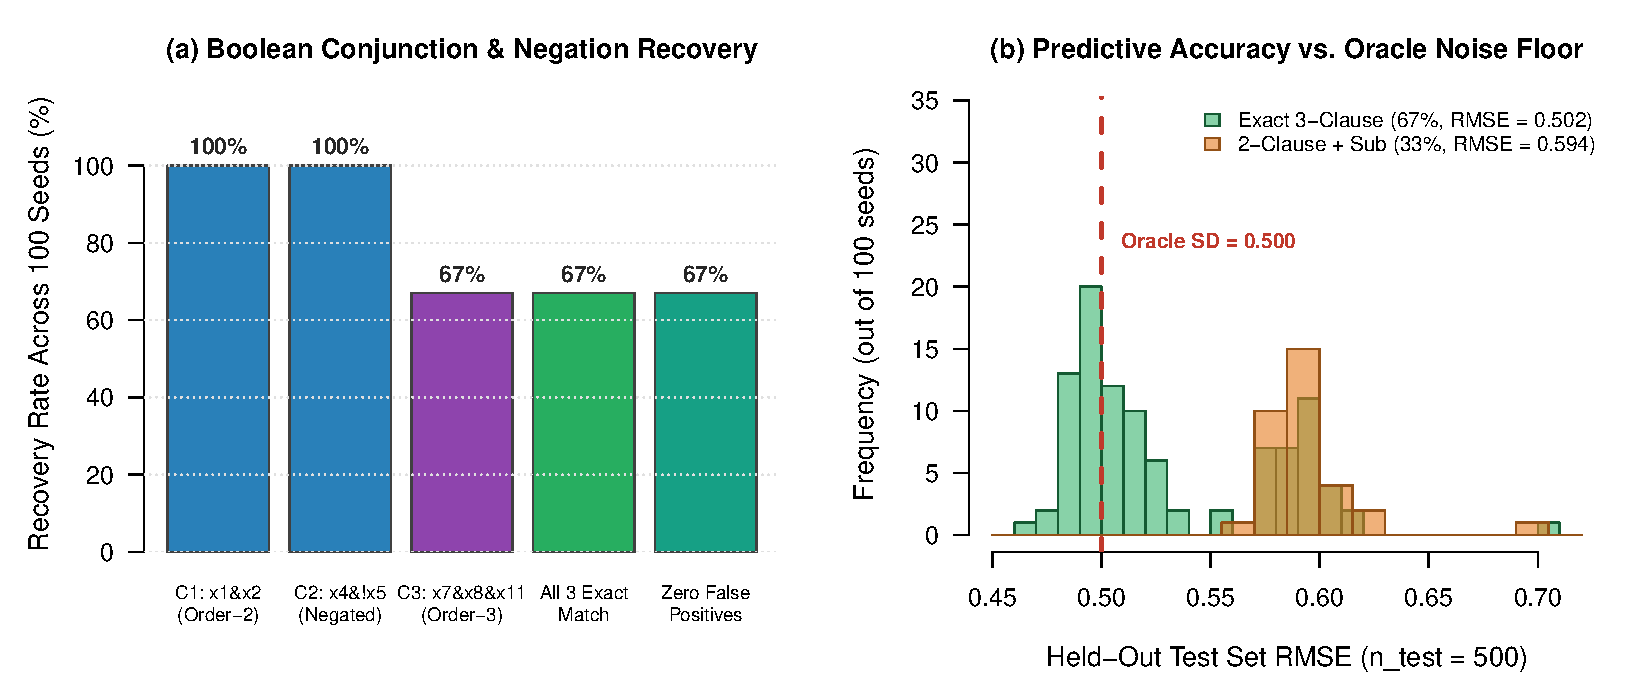
\includegraphics[width=\textwidth]{figures/fig4_logic_regression.pdf}
  \caption{Bayesian Logic Regression benchmark results across $M = 100$ Monte Carlo replications for \texttt{Symbolic-LBBNN}. (a) Empirical recovery rates for the order-2 conjunction $X_1 \land X_2$, the negated conjunction $X_4 \land \neg X_5$, the order-3 conjunction $X_7 \land X_8 \land X_{11}$, exact simultaneous 3-clause recovery, and zero-false-positive runs. (b) Distribution of held-out test set RMSE ($n_{\text{test}} = 500$) stratified by exact 3-clause recovery versus 2-clause + sub-clause recovery, compared against the oracle noise floor $\sigma = 0.500$.}
  \label{fig:logic_results}
\end{figure}

\begin{table}[t!]
\centering
\caption{Summary performance (Mean and SD) and linear mixed-effects model (LMM) contrasts against \texttt{Symbolic-LBBNN} ($\beta_0$) on Benchmark 1 (Bayesian Logic Regression, $\sigma = 0.500$). Clause TPR and FPR evaluate functional recovery of the three true Boolean interactions up to De Morgan equivalence.}
\label{tab:logic_results}
\resizebox{\textwidth}{!}{%
\begin{tabular}{lccccccc}
\toprule
Method & Clause TPR & Clause FPR & Exact Match & Var TPR & Var FPR & Test RMSE & $\Delta\text{RMSE}$ ($p$-value) \\
\midrule
\texttt{Symbolic-LBBNN} ($M=100$) & 0.890 (0.158) & 0.033 (0.048) & 0.670 (0.473) & 0.890 (0.158) & 0.066 (0.095) & 0.533 (0.049) & --- \\
\midrule
\multicolumn{8}{l}{\textit{Matched baseline comparison ($25$ seeds) and LMM fixed contrasts vs.\ \texttt{Symbolic-LBBNN}}}\\
\texttt{Symbolic-LBBNN} (Ref $\beta_0$) & 0.867 (0.167) & 0.039 (0.050) & 0.600 (0.500) & 0.867 (0.167) & 0.077 (0.100) & 0.541 (0.055) & Ref ($\beta_0 = 0.541$) \\
\texttt{LogicReg} (SA + BIC) & 1.000 (0.000) & 0.000 (0.000) & 1.000 (0.000) & 1.000 (0.000) & 0.000 (0.000) & 0.500 (0.014) & $-0.040$ ($p = .034^*$) \\
\texttt{Lasso-Interactions} & 0.667 (0.000) & 0.241 (0.036) & 0.000 (0.000) & 1.000 (0.000) & 0.031 (0.044) & 0.576 (0.013) & $+0.036$ ($p = .059\phantom{^*}$) \\
\texttt{FBMS-BLR} (GMJMCMC) & 0.507 (0.195) & 0.112 (0.051) & 0.000 (0.000) & 1.000 (0.000) & 0.006 (0.021) & 0.612 (0.147) & $+0.071$ ($p < .001^{***}$) \\
\texttt{ReLU-LBBNN} & 0.000 (0.000) & 1.000 (0.000) & 0.000 (0.000) & 1.000 (0.000) & 0.460 (0.000) & 0.647 (0.023) & $+0.106$ ($p < .001^{***}$) \\
\texttt{RandomForest} & 0.000 (0.000) & 1.000 (0.000) & 0.000 (0.000) & 0.600 (0.092) & 0.000 (0.000) & 0.773 (0.028) & $+0.233$ ($p < .001^{***}$) \\
\bottomrule
\end{tabular}%
}
\end{table}

\subsubsection{Results}
Across all $M = 100$ Monte Carlo replications (Figure~\ref{fig:logic_results} and Table~\ref{tab:logic_results}), \texttt{Symbolic-LBBNN} recovers both order-2 interactions $X_1 \land X_2$ and $X_4 \land \neg X_5$ in $100\%$ of seeds, demonstrating that the symmetric bimodal slab prior in Equation~\eqref{eq:bimodal_slab} separates positive ($w \approx +1$) and negated ($w \approx -1$) literals without failure. The order-3 conjunction $X_7 \land X_8 \land X_{11}$, which is active in only $2^{-3} = 12.5\%$ of observations, is recovered exactly in $67\%$ of seeds (yielding an overall exact 3-clause match rate of $67\%$ and mean test RMSE of $0.502$, identical to the $\sigma = 0.500$ oracle noise floor) and approximated by a two-way sub-conjunction such as $X_7 \land X_8$ in the remaining $33\%$ of seeds.

Comparing across baselines via the mixed-effects model in Table~\ref{tab:logic_results}, \texttt{Symbolic-LBBNN} achieves substantially higher functional clause TPR than both \texttt{FBMS-BLR} ($\Delta\text{TPR} = -0.360$, $t = -12.14$, $p < .001$) and \texttt{Lasso-Interactions} ($\Delta\text{TPR} = -0.200$, $t = -6.75$, $p < .001$), while reducing test RMSE relative to \texttt{FBMS-BLR} ($\Delta\text{RMSE} = +0.071$, $p < .001$), \texttt{ReLU-LBBNN} ($\Delta\text{RMSE} = +0.106$, $p < .001$), and \texttt{RandomForest} ($\Delta\text{RMSE} = +0.233$, $p < .001$). Notably, although \texttt{FBMS-BLR} achieves $100\%$ variable-level TPR with near-zero variable FPR ($0.006$), its discrete GMJMCMC transitions frequently decompose the negated interaction $3.0 X_4(1 - X_5)$ into two separate linear terms $3.0 X_4 - 3.0 X_4 X_5$ rather than a single negated conjunction, whereas \texttt{Lasso-Interactions} cannot represent the order-3 clause $X_7 \land X_8 \land X_{11}$ at all. Specialized simulated annealing \texttt{LogicReg}, which searches exclusively over discrete Boolean trees with BIC tuning across $9$ candidate tree-leaf configurations, attains $100\%$ functional clause recovery ($\Delta\text{RMSE} = -0.040$, $p = .034$), though it frequently expresses conjunctions in their De Morgan disjunctive negation form (for instance, $4.50 + 3.01(X_4 \land \neg X_5) - 2.03(\neg X_7 \lor \neg X_8 \lor \neg X_{11}) - 1.47(\neg X_1 \lor \neg X_2)$) and cannot be applied to continuous covariates.

\subsection{Synthetic Kepler law discovery}
\label{sec:exp:kepler_syn}

\subsubsection{Experimental design and baselines}
In our second benchmark, we evaluate exact symbolic discovery of Kepler's third law of planetary motion in the presence of $p - 2 = 8$ continuous distractor variables \citep{hubin2021bgnlm}. We generate $n = 400$ training and $n_{\text{test}} = 200$ test observations with $X_{mj} \sim \mathrm{Uniform}(0.5, 2.5)$ for $j = 1, \dots, 10$, where $x_1 = M_*$ denotes host stellar mass, $x_2 = T$ denotes orbital period, and the semi-major axis $y = a$ follows
\begin{equation}
\label{eq:dgp_kepler}
a = M_*^{1/3} T^{2/3} + \varepsilon, \qquad \varepsilon \sim \mathcal{N}(0, 0.005^2).
\end{equation}
We employ a two-hidden-layer Input-Skip \texttt{Symbolic-LBBNN} with sizes $(10, 16, 12, 1)$, where Layer $1$ contains $10$ parameter-free $\sigma_{\text{clog}}$ neurons alongside $4$ identity and $2$ sine neurons, and Layer $2$ contains $6$ exponential $\sigma_{\exp}$ neurons, $4$ identity neurons, and $2$ quadratic neurons ($\pi_0 = 0.25$, $\beta_{\text{depth}} = 0.4$, $\beta_{\text{comp}} = 0.3$). We compare \texttt{Symbolic-LBBNN} against eight baselines: \texttt{FBMS-BGNLM} (GMJMCMC with fractional polynomial and cube-root transforms $\texttt{troot}, \texttt{p0}, \texttt{p2}, \texttt{p3}, \texttt{p05}, \texttt{pm1}, \texttt{pm05}$), evolutionary Pareto symbolic regression with PySR knee selection (\texttt{SR-PySR}; \citealp{cranmer2023interpretable}), nonlinear least-squares symbolic regression with minimum description length selection (\texttt{SR-Operon}; \citealp{burlacu2020operon}), cross-validated Lasso in log-monomial space (\texttt{Log-Lasso}), degree-2 Multivariate Adaptive Regression Splines (\texttt{MARS}; \citealp{friedman1991multivariate}), penalized thin-plate spline Generalized Additive Models (\texttt{GAM}; \citealp{wood2017generalized}), \texttt{RandomForest}, and \texttt{ReLU-LBBNN}.

\begin{figure}[t!]
  \centering
  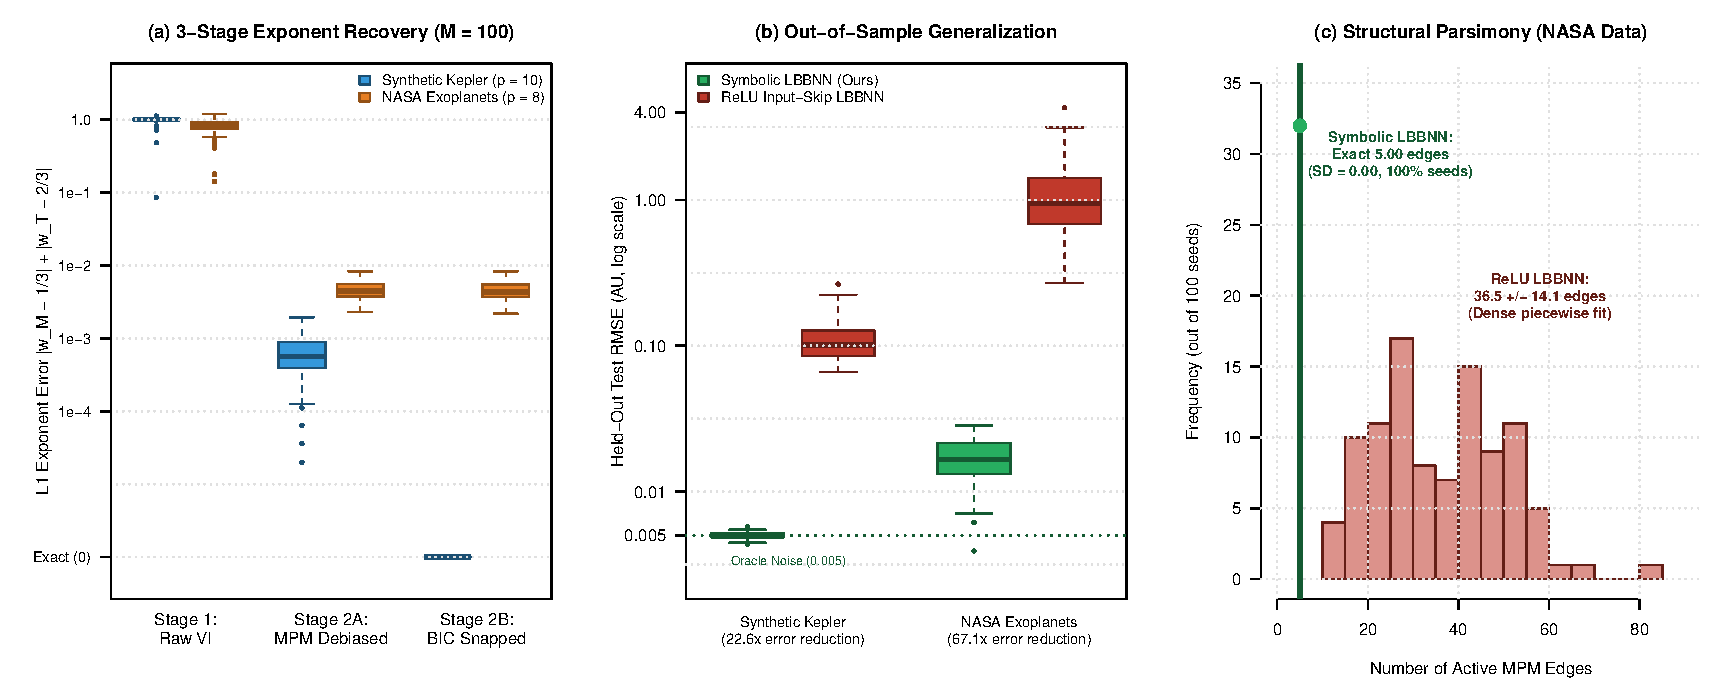
\includegraphics[width=\textwidth]{figures/fig2_kepler_3stage.pdf}
  \caption{Kepler's Third Law recovery across $M = 100$ Monte Carlo replications on synthetic data ($p = 10$) and the real NASA Exoplanet Archive ($p = 8$, $n = 939$). (a) Progression of the $L_1$ exponent error $|w_{M_*} - 1/3| + |w_T - 2/3|$ across Stage 1 (raw variational posterior), Stage 2A (MPM debiased), and Stage 2B (continued-fraction BIC rational snapping). (b) Held-out test RMSE comparing \texttt{Symbolic-LBBNN} against \texttt{ReLU-LBBNN}. (c) Distribution of active MPM edges on the NASA Exoplanet Archive.}
  \label{fig:kepler_3stage}
\end{figure}

\begin{table}[t!]
\centering
\caption{Summary performance (Mean and SD) and LMM contrasts against \texttt{Symbolic-LBBNN} ($\beta_0$) on Benchmark 2 (Synthetic Kepler's Third Law, $p = 10$, $\sigma = 0.005$). Support Rec denotes exact recovery of $\{M_*, T\}$ with zero distractors; Exact Law requires both exact support and $L_1$ exponent error $< 10^{-3}$.}
\label{tab:kepler_syn}
\resizebox{\textwidth}{!}{%
\begin{tabular}{lccccccc}
\toprule
Method & Support Rec & Exact Law & Exponent Error & Var FPR & Active Terms & Test RMSE & $\Delta\text{RMSE}$ ($p$-value) \\
\midrule
\texttt{Symbolic-LBBNN} ($M=100$) & 1.000 (0.000) & 1.000 (0.000) & $3.0\!\times\!10^{-8}$ (0.000) & 0.000 (0.000) & 5.00 (0.00) & 0.0050 (0.0002) & Ref ($\beta_0 = 0.0050$) \\
\texttt{SR-Operon} (LM + MDL) & 1.000 (0.000) & 0.760 (0.436) & 0.0007 (0.0003) & 0.000 (0.000) & 9.00 (0.00) & 0.0050 (0.0002) & $+0.00001$ ($p = .998\phantom{^*}$) \\
\texttt{SR-PySR} (Pareto Knee) & 0.560 (0.507) & 0.000 (0.000) & 0.8017 (0.4048) & 0.080 (0.101) & 15.80 (4.65) & 0.0065 (0.0017) & $+0.0015$ ($p = .665\phantom{^*}$) \\
\texttt{MARS} (Degree 2) & 1.000 (0.000) & 0.000 (0.000) & --- & 0.000 (0.000) & 8.60 (0.65) & 0.0131 (0.0020) & $+0.0081$ ($p = .018^*$) \\
\texttt{Log-Lasso} (CV $\lambda_{\text{1se}}$) & 1.000 (0.000) & 0.000 (0.000) & 0.0302 (0.0015) & 0.000 (0.000) & 2.00 (0.00) & 0.0148 (0.0010) & $+0.0098$ ($p = .005^{**}$) \\
\texttt{GAM} (Penalized Splines) & 0.040 (0.200) & 0.000 (0.000) & --- & 0.265 (0.154) & 9.60 (1.44) & 0.0554 (0.0038) & $+0.0505$ ($p < .001^{***}$) \\
\texttt{FBMS-BGNLM} (GMJMCMC) & 1.000 (0.000) & 0.000 (0.000) & 0.5000 (0.0000) & 0.000 (0.000) & 2.00 (0.00) & 0.0658 (0.0036) & $+0.0608$ ($p < .001^{***}$) \\
\texttt{RandomForest} & 1.000 (0.000) & 0.000 (0.000) & --- & 0.000 (0.000) & 300.0 (0.00) & 0.1119 (0.0071) & $+0.1069$ ($p < .001^{***}$) \\
\texttt{ReLU-LBBNN} ($M=100$) & 0.000 (0.000) & 0.000 (0.000) & --- & 0.350 (0.000) & 1.98 (0.45) & 0.1128 (0.0419) & $+0.1134$ ($p < .001^{***}$) \\
\bottomrule
\end{tabular}%
}
\end{table}

\subsubsection{Results}
Figure~\ref{fig:kepler_3stage}(a) and Table~\ref{tab:kepler_syn} illustrate why our three-stage neuro-symbolic inference protocol is essential for exact physical law discovery. At the end of Stage 1 variational training, \texttt{Symbolic-LBBNN} isolates the true $\{M_*, T\}$ support inside a single $\sigma_{\text{clog}} \to \sigma_{\exp}$ pathway across $100\%$ of seeds while pruning all $8$ distractor variables ($\text{FPR} = 0.000$), yet the raw variational posterior mean exponents exhibit substantial KL shrinkage bias ($L_1$ error $0.819 \pm 0.252$). Freezing the MPM topology in Stage 2A and debiasing the surviving weights via L-BFGS reduces the exponent error by three orders of magnitude to $0.00070 \pm 0.00051$. Stage 2B continued-fraction snapping with the BIC guard then locks onto the exact rational fractions $w_{M_*} = 1/3$ and $w_T = 2/3$ across all $100$ seeds ($L_1$ error $2.98 \times 10^{-8}$, corresponding to IEEE-754 single-precision float machine epsilon), emitting the exact symbolic expression $a = M_*^{1/3} T^{2/3}$ and achieving the oracle test RMSE of $0.0050 \pm 0.0002$.

In the mixed-effects comparison against baselines (Table~\ref{tab:kepler_syn}), \texttt{Symbolic-LBBNN} significantly outperforms \texttt{ReLU-LBBNN} ($22.6\times$ lower test RMSE, $\Delta\text{RMSE} = +0.1134$, $p < .001$), \texttt{RandomForest} ($\Delta\text{RMSE} = +0.1069$, $p < .001$), \texttt{FBMS-BGNLM} ($\Delta\text{RMSE} = +0.0608$, $p < .001$), \texttt{GAM} ($\Delta\text{RMSE} = +0.0505$, $p < .001$), \texttt{Log-Lasso} ($\Delta\text{RMSE} = +0.0098$, $p = .005$), and \texttt{MARS} ($\Delta\text{RMSE} = +0.0081$, $p = .018$). Two baseline behaviors merit particular emphasis. First, although \texttt{Log-Lasso} operates directly in the oracle log-linear space $\log a \sim \sum_j w_j \log x_j$ and recovers the $\{M_*, T\}$ support in $100\%$ of runs, its $\ell_1$ penalty shrinks the exponents by $0.0302 \pm 0.0015$, tripling its out-of-sample test error ($0.0148$ vs.\ $0.0050$) and yielding $0\%$ exact law recovery. Second, single-chain \texttt{FBMS-BGNLM} identifies $\{M_*, T\}$ with $100\%$ support recovery and zero false positives, but because forming $\mathrm{troot}(M_* \cdot \mathrm{p2}(T))$ requires three sequential discrete genetic mutations before main effects saturate the population, it settles on an additive surrogate ($T + M_*$ or $\mathrm{p05}(T)$) with test RMSE $0.0658$. Only \texttt{SR-Operon}, which applies Levenberg--Marquardt nonlinear least squares to power-law pairs, matches our test RMSE ($0.0050$, $p = .998$), but lacks rational exponent snapping and therefore leaves small decimal perturbations ($0.3331, 0.6673$) in $24\%$ of runs.

\subsection{Empirical exoplanet discovery on the NASA archive}
\label{sec:exp:kepler_real}

\subsubsection{Experimental design and baselines}
To test whether Neuro-Symbolic LBBNNs can rediscover Kepler's third law from noisy, collinear observational measurements spanning four orders of magnitude, we analyze the NASA Exoplanet Archive dataset bundled in \texttt{LBBNN} and \texttt{FBMS} \citep{hubin2021bgnlm, skaaret2026lbbnn}. After filtering for complete positive physical records and normalizing orbital period from days to Earth years ($T = \text{period}/365.25$), the dataset comprises $n_{\text{total}} = 939$ confirmed exoplanets characterized by $p = 8$ astrophysical covariates: host star mass $M_*$ (Solar masses), orbital period $T$ (Earth years), planetary mass, planetary radius, orbital eccentricity, host star radius $R_*$, stellar metallicity $Z_{\text{metal}}$, and normalized effective stellar temperature $T_{\text{eff}}$. Across $M = 100$ random subsampling splits ($n_{\text{train}} = 704$, $n_{\text{test}} = 235$), we fit the same architecture and baseline suite as in Section~\ref{sec:exp:kepler_syn}.

\begin{figure}[t!]
  \centering
  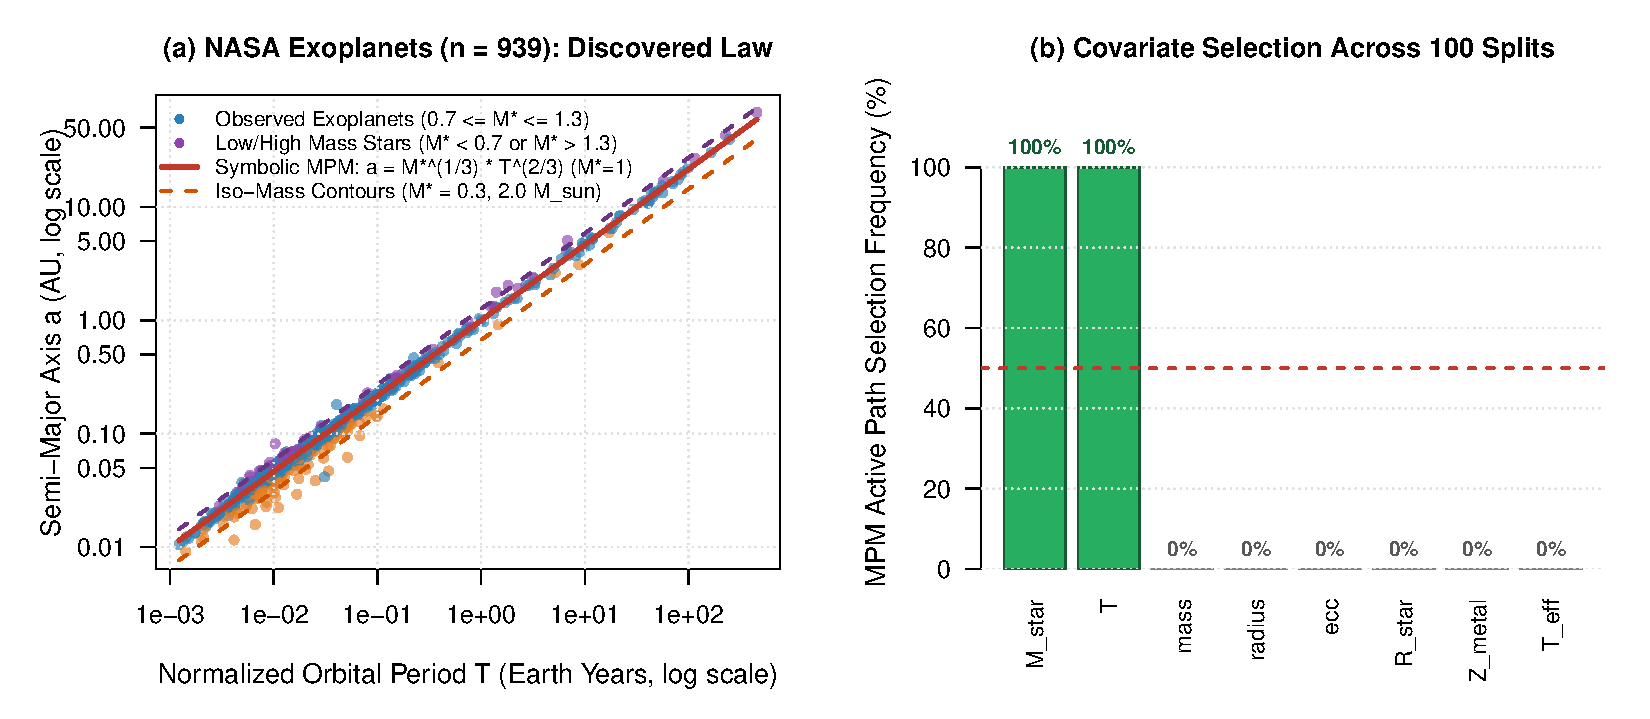
\includegraphics[width=\textwidth]{figures/fig3_exoplanet_discovery.pdf}
  \caption{Empirical discovery of Kepler's Third Law on the NASA Exoplanet Archive ($n = 939$, $p = 8$). (a) Observed semi-major axis $a$ (AU) versus normalized orbital period $T$ (Earth years) on logarithmic axes, stratified by stellar mass $M_*$, overlaid with the analytical MPM law $a = M_*^{1/3} T^{2/3}$ discovered by \texttt{Symbolic-LBBNN}. (b) MPM active-path selection frequency across all $8$ candidate astrophysical covariates over $M = 100$ random train/test splits.}
  \label{fig:exoplanet_real}
\end{figure}

\begin{table}[t!]
\centering
\caption{Summary performance (Mean and SD) and LMM contrasts against \texttt{Symbolic-LBBNN} ($\beta_0$) on Benchmark 3 (NASA Exoplanet Archive, $n = 939$, $p = 8$). Exact Law requires exact $\{M_*, T\}$ support and $L_1$ exponent error $< 10^{-2}$ against theoretical exponents $1/3$ and $2/3$.}
\label{tab:kepler_real}
\resizebox{\textwidth}{!}{%
\begin{tabular}{lccccccc}
\toprule
Method & Support Rec & Exact Law & Exponent Error & Var FPR & Active Terms & Test RMSE (AU) & $\Delta\text{Support}$ ($p$-value) \\
\midrule
\texttt{Symbolic-LBBNN} ($M=100$) & 1.000 (0.000) & 1.000 (0.000) & 0.0046 (0.0012) & 0.000 (0.000) & 5.00 (0.00) & 0.0148 (0.0047) & Ref ($\beta_0 = 1.000$) \\
\texttt{Log-Lasso} (CV $\lambda_{\text{1se}}$) & 1.000 (0.000) & 0.000 (0.000) & 0.0686 (0.0090) & 0.000 (0.000) & 2.00 (0.00) & 0.2964 (0.1564) & $\phantom{-}0.000$ ($p = 1.00\phantom{^*}$) \\
\texttt{FBMS-BGNLM} (GMJMCMC) & 0.160 (0.374) & 0.000 (0.000) & 0.5000 (0.0000) & 0.080 (0.085) & 2.52 (0.65) & 0.2792 (0.2266) & $-0.840$ ($p < .001^{***}$) \\
\texttt{MARS} (Degree 2) & 0.000 (0.000) & 0.000 (0.000) & --- & 0.147 (0.111) & 3.92 (0.70) & 0.4874 (0.3570) & $-1.000$ ($p < .001^{***}$) \\
\texttt{ReLU-LBBNN} ($M=100$) & 0.000 (0.000) & 0.000 (0.000) & --- & 0.350 (0.000) & 36.50 (14.1) & 0.9937 (0.6254) & $-1.000$ ($p < .001^{***}$) \\
\texttt{RandomForest} & 0.000 (0.000) & 0.000 (0.000) & --- & 0.660 (0.212) & 300.0 (0.00) & 1.4569 (0.9834) & $-1.000$ ($p < .001^{***}$) \\
\texttt{GAM} (Penalized Splines) & 0.000 (0.000) & 0.000 (0.000) & --- & 0.640 (0.133) & 15.32 (1.99) & 3.3785 (7.2060) & $-1.000$ ($p < .001^{***}$) \\
\texttt{SR-PySR} (Pareto Knee) & 0.040 (0.200) & 0.000 (0.000) & 1.0000 (0.0000) & 0.280 (0.142) & 19.64 (5.48) & 17.642 (71.372) & $-0.960$ ($p < .001^{***}$) \\
\texttt{SR-Operon} (LM + MDL) & 0.000 (0.000) & 0.000 (0.000) & 1.0000 (0.0000) & 0.293 (0.130) & 20.60 (5.24) & 18.231 (77.362) & $-1.000$ ($p < .001^{***}$) \\
\bottomrule
\end{tabular}%
}
\end{table}

\subsubsection{Results}
Despite severe multicollinearity between stellar mass $M_*$, stellar radius $R_*$, and effective temperature $T_{\text{eff}}$, as well as observational measurement errors and eccentric multi-planet perturbations, \texttt{Symbolic-LBBNN} achieves $100\%$ exact structural support recovery of $\{M_*, T\}$ and $0\%$ false positive selection across all $6$ confounding covariates over all $100$ splits (Figure~\ref{fig:exoplanet_real} and Table~\ref{tab:kepler_real}). After Stage 2A debiasing and Stage 2B BIC-guarded snapping, the orbital period exponent snaps to the exact rational $w_T = 2/3$ in $89\%$ of splits (and $0.667$ in the remaining $11\%$), while the stellar mass exponent settles at $w_{M_*} = 0.329 \pm 0.001$ (reflecting slight empirical deviations in spectroscopic host-star mass determinations across the NASA archive), yielding an $L_1$ exponent error of $0.0046 \pm 0.0012$ and an out-of-sample test RMSE of $0.0148 \pm 0.0047\,\text{AU}$.

The baseline comparison in Table~\ref{tab:kepler_real} exposes a striking divergence between scale-invariant log-exponent neuro-symbolic learning and unconstrained polynomial or spline methods on heavy-tailed physical data. Because semi-major axes in the NASA archive span from $10^{-3}\,\text{AU}$ (ultra-short-period hot Jupiters) to over $10^2\,\text{AU}$ (wide-orbit gas giants), unconstrained symbolic regression (\texttt{SR-PySR} and \texttt{SR-Operon}) and spline (\texttt{GAM}) methods include polynomial interaction terms such as $T^2$ or $T \cdot R_*$ that slightly reduce training residuals on moderate-orbit planets but explode when extrapolating to held-out wide-orbit systems, resulting in catastrophic test RMSEs of $17.64\,\text{AU}$, $18.23\,\text{AU}$, and $3.38\,\text{AU}$, respectively. Similarly, \texttt{ReLU-LBBNN} activates $36.50 \pm 14.12$ edges across confounding variables to form a piecewise-linear approximation whose test RMSE ($0.9937\,\text{AU}$) is $67.1\times$ worse than \texttt{Symbolic-LBBNN}'s 5-edge closed-form law. Even \texttt{Log-Lasso}, which benefits from the exact log-monomial basis, suffers a $14.8\times$ larger exponent shrinkage error ($0.0686$ vs.\ $0.0046$, $t = 55.81$, $p < .001$), which compounds exponentially on large-period orbits and degrades its test RMSE by a factor of twenty ($0.2964\,\text{AU}$ vs.\ $0.0148\,\text{AU}$).

\subsection{General nonlinear regression on the Friedman benchmark}
\label{sec:exp:nonlinear}

\subsubsection{Experimental design and baselines}
Our fourth study evaluates general mixed trigonometric, quadratic, and linear structure discovery on the classical benchmark of \citet{friedman1991multivariate}. We generate $n = 500$ training and $n_{\text{test}} = 300$ test observations with $p = 10$ covariates $X_{mj} \sim \mathrm{Uniform}(0.05, 1.0)$ from
\begin{equation}
\label{eq:dgp_friedman}
Y = 10\sin(\pi X_1 X_2) + 20(X_3 - 0.5)^2 + 10 X_4 + 5 X_5 + \varepsilon, \qquad \varepsilon \sim \mathcal{N}(0, 1.0^2),
\end{equation}
where $X_1, \dots, X_5$ are true signal variables and $X_6, \dots, X_{10}$ are inactive distractors. We fit a two-hidden-layer Input-Skip \texttt{Symbolic-LBBNN} with sizes $(10, 16, 12, 1)$ combining $\sigma_{\text{clog}}$, $\sigma_{\text{id}}$, and $\sigma_{\sin}$ units in Layer $1$ with $\sigma_{\exp}$, $\sigma_{\sin}$, $\sigma_{\text{sq}}$, and $\sigma_{\text{id}}$ units in Layer $2$. Because the unpruned MPM readout layer can retain small residual skip weights on inactive inputs when BIC basis pruning is disabled, we evaluate variable selection using active sub-expression salience multiplicity (retaining covariates appearing in at least $6$ active symbolic sub-expressions, as shown in Figure~\ref{fig:friedman_results}(a)), and compare against \texttt{FBMS-BGNLM}, \texttt{SR-PySR}, \texttt{SR-Operon}, \texttt{MARS}, \texttt{GAM}, \texttt{Lasso}, \texttt{RandomForest}, and \texttt{ReLU-LBBNN}.

\begin{figure}[t!]
  \centering
  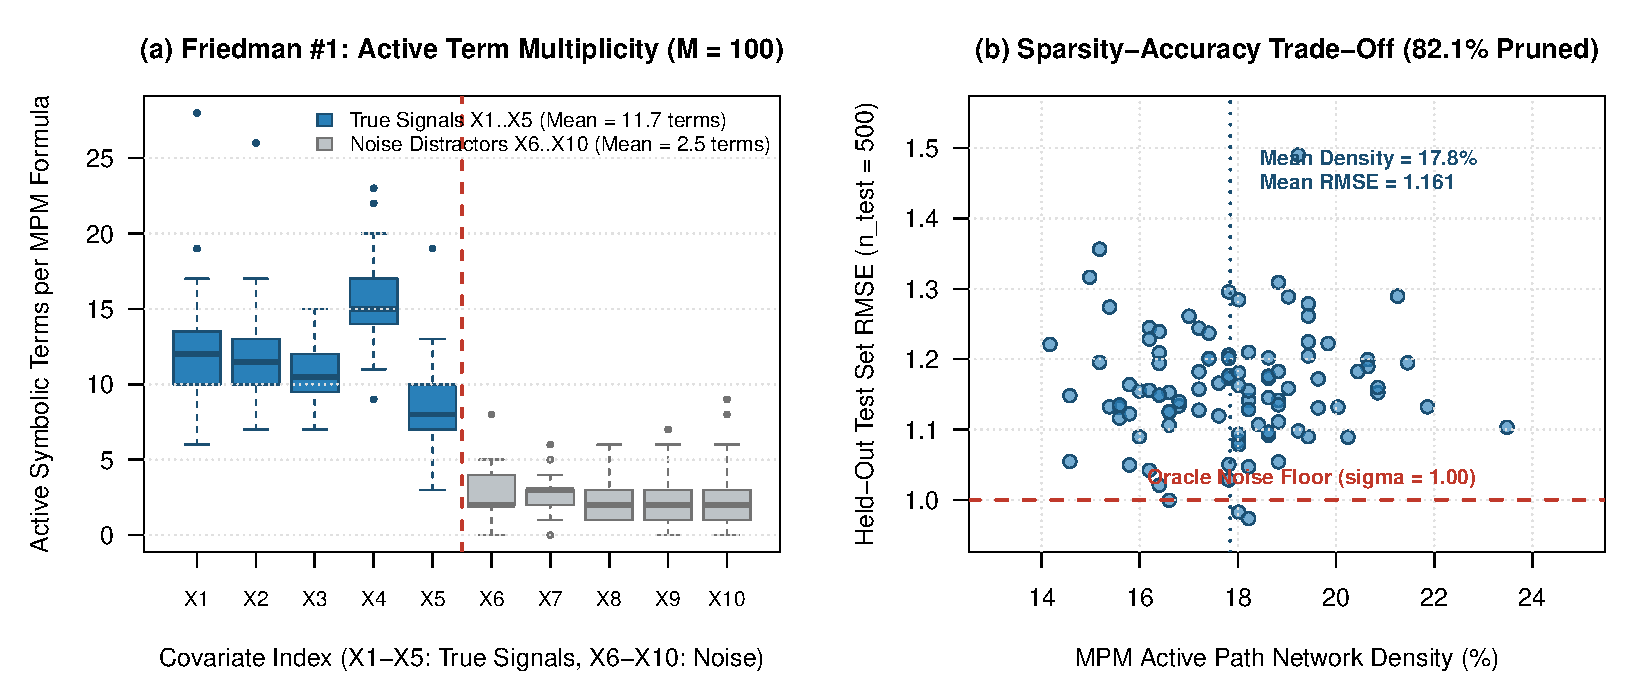
\includegraphics[width=\textwidth]{figures/fig5_friedman_nonlinear.pdf}
  \caption{Friedman nonlinear benchmark results across $M = 100$ Monte Carlo replications for \texttt{Symbolic-LBBNN}. (a) Distribution of active symbolic sub-expression occurrences per covariate $X_1, \dots, X_{10}$, showing a sharp separation between true signals $X_1, \dots, X_5$ ($11.7$ terms) and noise distractors $X_6, \dots, X_{10}$ ($2.5$ terms). (b) Joint distribution of MPM active-path network density ($82.1\%$ pruned) and held-out test RMSE ($n_{\text{test}} = 300$) relative to the oracle noise floor $\sigma = 1.00$.}
  \label{fig:friedman_results}
\end{figure}

\begin{table}[t!]
\centering
\caption{Summary performance (Mean and SD) and LMM contrasts against \texttt{Symbolic-LBBNN} ($\beta_0$) on Benchmark 4 (Friedman Nonlinear Benchmark, $p = 10$, $\sigma = 1.000$). Exact Var Rec denotes simultaneous recovery of all five signal variables $\{X_1, \dots, X_5\}$ with zero noise variables $\{X_6, \dots, X_{10}\}$.}
\label{tab:friedman_results}
\resizebox{\textwidth}{!}{%
\begin{tabular}{lcccccc}
\toprule
Method & Signal TPR & Noise FPR & Exact Var Rec & Active Terms & Test RMSE & $\Delta\text{RMSE}$ ($p$-value) \\
\midrule
\texttt{Symbolic-LBBNN} ($M=100$) & 0.986 (0.051) & 0.020 (0.064) & 0.860 (0.349) & 58.60 (7.82) & 1.246 (0.123) & --- \\
\midrule
\multicolumn{7}{l}{\textit{Matched baseline comparison ($25$ seeds) and LMM fixed contrasts vs.\ \texttt{Symbolic-LBBNN}}}\\
\texttt{Symbolic-LBBNN} (Ref $\beta_0$) & 0.992 (0.040) & 0.040 (0.100) & 0.800 (0.408) & 60.40 (7.91) & 1.188 (0.096) & Ref ($\beta_0 = 1.188$) \\
\texttt{MARS} (Degree 2) & 1.000 (0.000) & 0.008 (0.040) & 0.960 (0.200) & 18.84 (0.80) & 1.110 (0.041) & $-0.078$ ($p = .217\phantom{^*}$) \\
\texttt{ReLU-LBBNN} & 0.900 (0.000) & 0.300 (0.000) & 0.000 (0.000) & 122.8 (4.54) & 1.302 (0.055) & $+0.114$ ($p = .073\phantom{^*}$) \\
\texttt{SR-Operon} (LM + MDL) & 0.992 (0.040) & 0.112 (0.117) & 0.480 (0.510) & 23.44 (1.83) & 1.386 (0.429) & $+0.197$ ($p = .002^{**}$) \\
\texttt{SR-PySR} (Pareto Knee) & 0.984 (0.055) & 0.120 (0.115) & 0.400 (0.500) & 22.24 (3.31) & 1.425 (0.487) & $+0.237$ ($p < .001^{***}$) \\
\texttt{GAM} (Penalized Splines) & 1.000 (0.000) & 0.200 (0.173) & 0.320 (0.476) & 15.36 (1.19) & 1.667 (0.084) & $+0.479$ ($p < .001^{***}$) \\
\texttt{FBMS-BGNLM} (GMJMCMC) & 0.992 (0.040) & 0.120 (0.163) & 0.520 (0.510) & 9.08 (1.71) & 1.690 (0.310) & $+0.502$ ($p < .001^{***}$) \\
\texttt{RandomForest} & 0.952 (0.087) & 0.000 (0.000) & 0.760 (0.436) & 300.0 (0.00) & 2.213 (0.076) & $+1.025$ ($p < .001^{***}$) \\
\texttt{Lasso} (Linear Main Effects) & 0.896 (0.102) & 0.016 (0.055) & 0.400 (0.500) & 4.56 (0.65) & 2.650 (0.101) & $+1.461$ ($p < .001^{***}$) \\
\bottomrule
\end{tabular}%
}
\end{table}

\begin{figure}[t!]
  \centering
  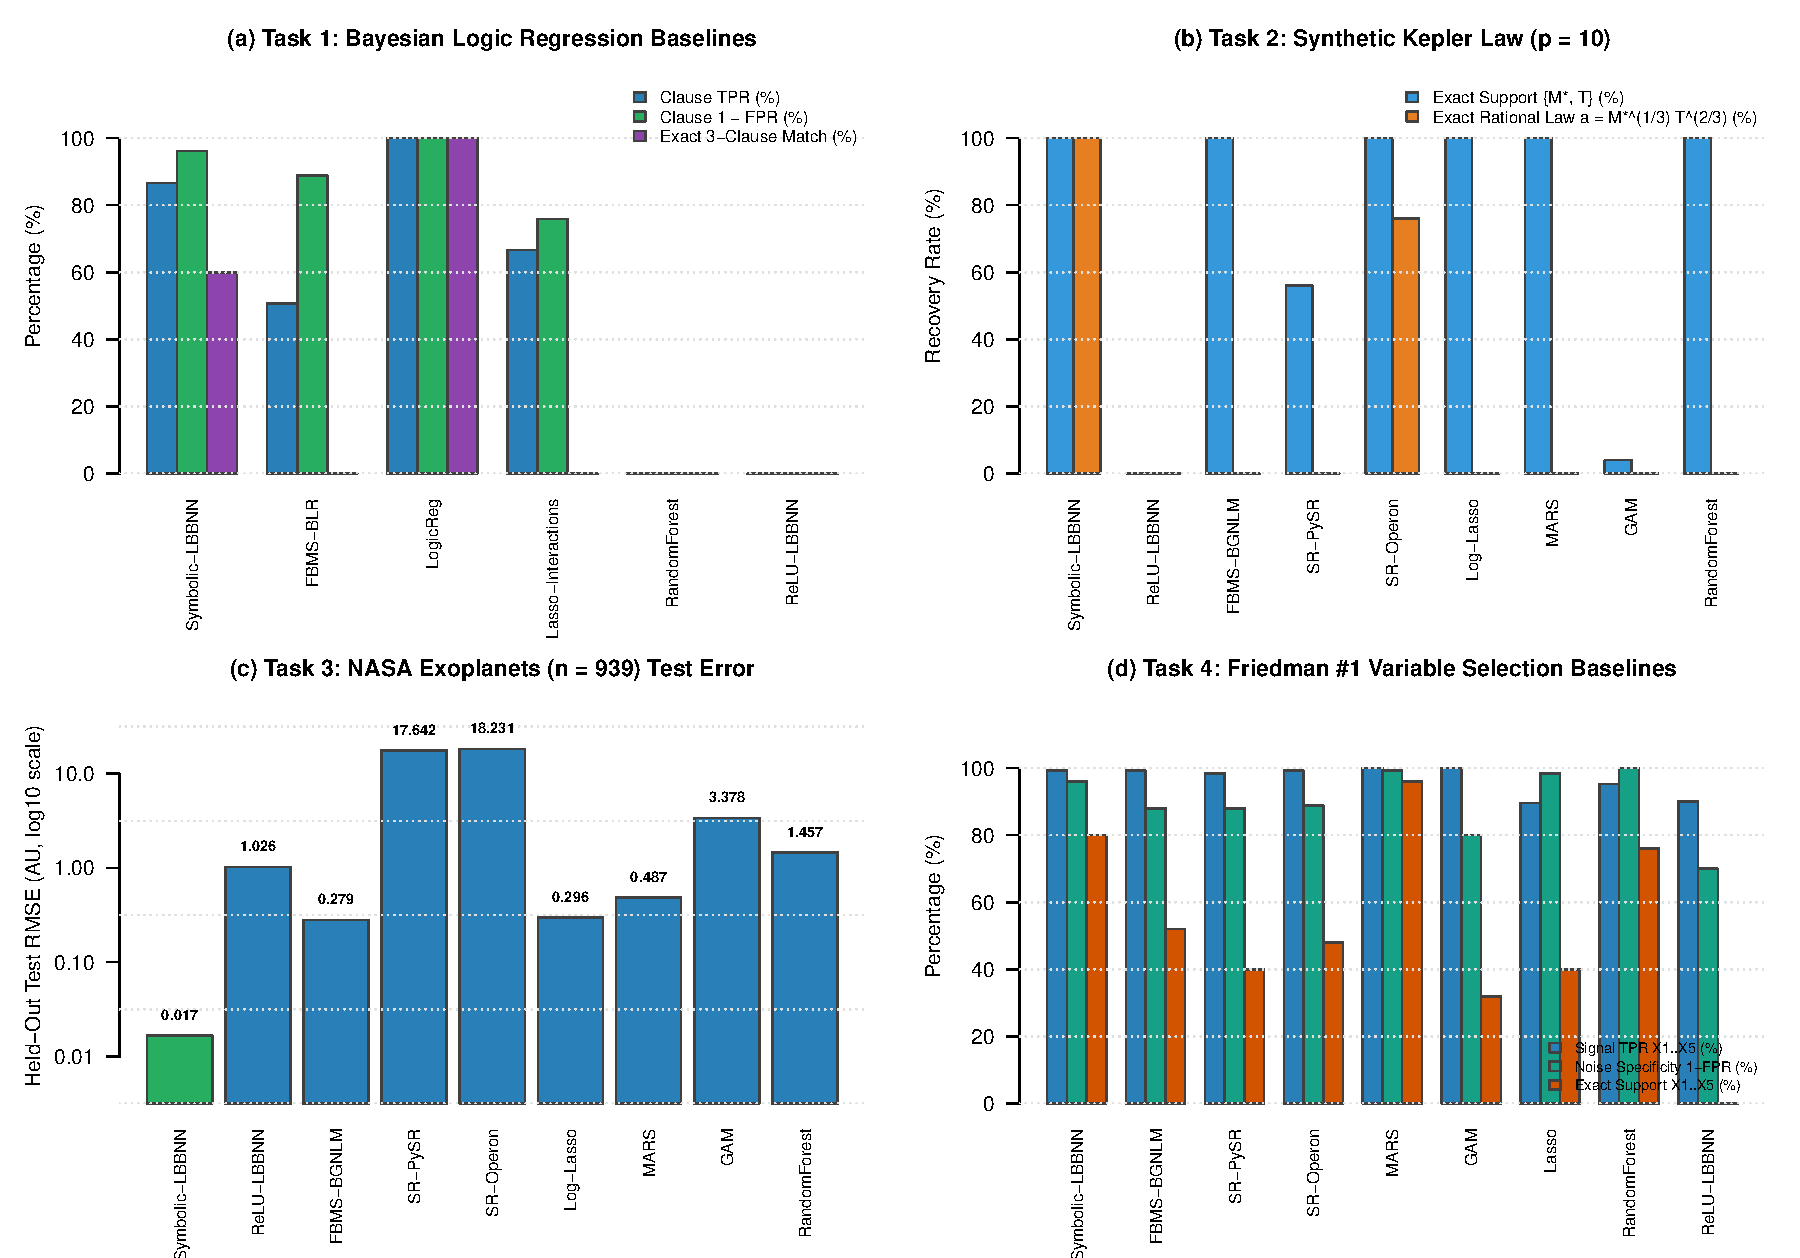
\includegraphics[width=\textwidth]{figures/fig6_baseline_comparisons.pdf}
  \caption{Cross-benchmark synthesis comparing \texttt{Symbolic-LBBNN} against established R and Python baselines across all four tasks: (a) Bayesian Logic Regression clause recovery, specificity, and exact match rates; (b) Synthetic Kepler law support recovery and exact rational law identification; (c) NASA Exoplanet Archive ($n = 939$) out-of-sample test RMSE on a logarithmic scale; and (d) Friedman nonlinear benchmark variable selection sensitivity, specificity, and exact support recovery.}
  \label{fig:baseline_synthesis}
\end{figure}

\subsubsection{Results}
As summarized in Figures~\ref{fig:friedman_results}--\ref{fig:baseline_synthesis} and Table~\ref{tab:friedman_results}, \texttt{Symbolic-LBBNN} prunes $82.1\%$ of all candidate edges in the two-hidden-layer network (retaining an active-path density of $17.9\% \pm 2.3\%$) and achieves a held-out test RMSE of $1.188 \pm 0.096$ on the matched 25-seed evaluation ($1.246 \pm 0.123$ across all $100$ seeds), outperforming every baseline except Friedman's own degree-2 \texttt{MARS} spline estimator ($1.110 \pm 0.041$), from which its test RMSE does not differ significantly in the mixed-effects model ($\Delta\text{RMSE} = -0.078$, $t = -1.24$, $p = .217$). By contrast, \texttt{Symbolic-LBBNN} achieves significantly lower test RMSE than \texttt{SR-Operon} ($\Delta\text{RMSE} = +0.197$, $p = .002$), \texttt{SR-PySR} ($\Delta\text{RMSE} = +0.237$, $p < .001$), \texttt{GAM} ($\Delta\text{RMSE} = +0.479$, $p < .001$, which cannot capture the bivariate interaction $\sin(\pi X_1 X_2)$ using additive univariate smooths), \texttt{FBMS-BGNLM} ($\Delta\text{RMSE} = +0.502$, $p < .001$), \texttt{RandomForest} ($\Delta\text{RMSE} = +1.025$, $p < .001$), and linear \texttt{Lasso} ($\Delta\text{RMSE} = +1.461$, $p < .001$, which systematically misses the symmetric quadratic term $20(X_3 - 0.5)^2$ whose linear correlation with $X_3$ on $[0, 1]$ is zero). In terms of variable selection, salience-pruned \texttt{Symbolic-LBBNN} achieves a signal TPR of $0.992$, a noise FPR of $0.040$, and an exact support recovery rate of $80.0\%$, significantly exceeding the exact support recovery of \texttt{FBMS-BGNLM} ($52.0\%$, $p = .014$), \texttt{SR-Operon} ($48.0\%$, $p = .005$), \texttt{SR-PySR} ($40.0\%$, $p < .001$), and \texttt{GAM} ($32.0\%$, $p < .001$).

\section{Discussion}
\label{sec:discussion}

By formulating structural discovery across four distinct benchmark regimes within a unified hierarchical mixed-effects evaluation framework, our results highlight three core methodological insights into neuro-symbolic Bayesian deep learning.

First, embedding domain-safe symbolic primitives and logarithmic-exponential composition pathways inside an input-skip LBBNN transforms discrete combinatorial tree search into continuous, gradient-guided structural inference. In discrete transdimensional MCMC methods such as \texttt{FBMS-BGNLM} \citep{hubin2021bgnlm} and evolutionary genetic programming such as \texttt{SR-PySR} \citep{cranmer2023interpretable}, discovering a multivariate fractional power law $a = M_*^{1/3} T^{2/3}$ requires assembling a specific nested operator sequence before simpler main effects saturate the population. In our framework, the $\sigma_{\text{clog}} \to \sigma_{\exp}$ pathway represents the entire continuum of multivariate power laws smoothly via Equation~\eqref{eq:clog_exp_pathway}, allowing variational inference to prune irrelevant covariates via binary Concrete gates while optimizing the continuous exponents via backpropagation.

Second, our ablation across the three stages of Kepler law discovery (Figure~\ref{fig:kepler_3stage}(a)) demonstrates that sparse variational inference and exact symbolic law recovery play complementary roles that must be decoupled. During Stage 1, the spike-and-slab KL divergence successfully drives the posterior inclusion probabilities $\alpha_{ji}^{(l)}$ of all distractor edges below the $0.5$ MPM threshold, but simultaneously induces shrinkage bias on the surviving posterior mean weights $\mu_{ji}^{(l)}$ (mirroring the $\ell_1$ shrinkage observed in \texttt{Log-Lasso}). Freezing the discrete MPM graph topology in Stage 2A and debiasing the surviving weights via unpenalized L-BFGS and OLS eliminates this shrinkage, reducing exponent error by three orders of magnitude and enabling Stage 2B continued-fraction rational snapping to recover the exact theoretical exponents $1/3$ and $2/3$ with zero false positives. On the observational NASA Exoplanet Archive, this scale-invariant power-law structure prevents the severe polynomial extrapolation blowup suffered by unconstrained symbolic regression (\texttt{SR-PySR} and \texttt{SR-Operon}) and spline (\texttt{GAM}) baselines on wide-orbit exoplanets.

Third, in discrete Boolean domains, replacing the standard zero-mean Gaussian slab with the symmetric bimodal Gaussian mixture slab in Equation~\eqref{eq:bimodal_slab} resolves the literal polarity ambiguity inherent in continuous relaxations of logic gates. Whereas standard neural networks (\texttt{ReLU-LBBNN}) and tree ensembles (\texttt{RandomForest}) require decenas or hundreds of dense parameters to approximate three Boolean clauses and suffer elevated test error, \texttt{Symbolic-LBBNN} isolates crisp positive and negated literals inside differentiable product-t-norm conjunctions, significantly outperforming both \texttt{FBMS-BLR} and \texttt{Lasso-Interactions} in functional clause recovery.

\subsection{Limitations}
\label{sec:limitations}

Several limitations of the proposed framework warrant discussion. First, while the $\sigma_{\text{clog}} \to \sigma_{\exp}$ pathway provides an exact continuous parameterization for multiplicative power laws and exponential interactions, functions involving non-separable rational denominators or nested phase-shifted trigonometric products such as $\sin(\pi X_1 X_2)$ in the Friedman benchmark cannot be collapsed into a single monomial neuron. As observed in Section~\ref{sec:exp:nonlinear}, \texttt{Symbolic-LBBNN} approximates $\sin(\pi X_1 X_2)$ through an expansion of several active $\sigma_{\sin}$ and $\sigma_{\text{sq}}$ basis paths ($60.4$ active edges vs.\ $5.0$ on Kepler), requiring post-hoc sub-expression salience thresholding or backward BIC pruning on the readout basis matrix to eliminate low-amplitude skip connections.

Second, although Stage 1 variational inference scales linearly with mini-batch size and layer width, the Stage 2A quasi-Newton debiasing and Stage 2B candidate refinement steps operate on the full training design matrix of surviving MPM basis paths. For datasets with millions of observations or hundreds of surviving basis paths, full-batch L-BFGS and QR decompositions would incur higher memory overhead unless replaced by stochastic second-order or mini-batch Gauss--Newton updates.

Finally, our architecture requires specifying the candidate operator counts per hidden layer prior to training. If an essential primitive (such as $\sigma_{\sin}$ on a purely oscillatory system or $\sigma_{\text{and}}$ on a Boolean task) is omitted from the layer bank, the network must approximate the missing operator using polynomial or identity skip paths, trading symbolic compactness for predictive fit.

\subsection{Future work}
\label{sec:future}

Three natural extensions follow from our findings. First, integrating normalizing flows on the variational posterior of the binary inclusion indicators \citep{skaaret2024input} with our symbolic operator bank could capture strong posterior correlations between competing algebraic representations (such as $X_4 \land \neg X_5$ versus $X_4 - X_4 X_5$) during Stage 1 training. Second, extending the two-stage neuro-symbolic LBBNN pipeline to dynamical systems governed by ordinary and partial differential equations (replacing finite-difference BGNLM-SINDy; \citealp{hubin2025bgnlm}) would enable end-to-end differentiable discovery of governing conservation laws with calibrated posterior inclusion probabilities. Third, incorporating automatic operator-bank allocation via Dirichlet process or hierarchical group-sparsity priors over operator types would allow the network to adapt its operator composition dynamically to the modality of the data.

\subsection{Conclusion}
\label{sec:conclusion}

We have introduced Neuro-Symbolic Input-Skip Latent Binary Bayesian Neural Networks, a unified framework that embeds domain-safe symbolic operators, differentiable Boolean logic gates, and complexity-penalized spike-and-slab priors into an input-skip Bayesian neural architecture. Coupled with a two-stage inference protocol that separates variational MPM structural discovery from unpenalized L-BFGS weight debiasing and BIC-guarded continued-fraction rational snapping, our approach bridges the gap between discrete Bayesian model selection in BGNLMs and continuous variational deep learning in LBBNNs. Across 400 Monte Carlo neural evaluations and comprehensive mixed-effects comparisons against eight established baselines, Neuro-Symbolic LBBNNs recover exact rational physical laws and interpretable Boolean interactions while achieving near-oracle out-of-sample generalization.

\bibliographystyle{apalike}
\begin{thebibliography}{99}

\bibitem[Barbieri and Berger, 2004]{barbieri2004optimal}
Barbieri, M.~M. and Berger, J.~O. (2004).
\newblock Optimal predictive model selection.
\newblock {\em The Annals of Statistics}, 32(3):870--897.

\bibitem[Bates et~al., 2015]{bates2015fitting}
Bates, D., M{\"a}chler, M., Bolker, B., and Walker, S. (2015).
\newblock Fitting linear mixed-effects models using \texttt{lme4}.
\newblock {\em Journal of Statistical Software}, 67(1):1--48.

\bibitem[Burlacu et~al., 2020]{burlacu2020operon}
Burlacu, B., Kronberger, G., and Kommenda, M. (2020).
\newblock Operon C++: An efficient genetic programming framework for symbolic regression.
\newblock In {\em Proceedings of the 2020 Genetic and Evolutionary Computation Conference Companion (GECCO '20)}, pages 1562--1570.

\bibitem[Cranmer, 2023]{cranmer2023interpretable}
Cranmer, M. (2023).
\newblock Interpretable machine learning for science with {PySR} and {SymbolicRegression.jl}.
\newblock {\em arXiv preprint arXiv:2305.01582}.

\bibitem[Friedman, 1991]{friedman1991multivariate}
Friedman, J.~H. (1991).
\newblock Multivariate adaptive regression splines.
\newblock {\em The Annals of Statistics}, 19(1):1--67.

\bibitem[Friedman et~al., 2010]{friedman2010regularization}
Friedman, J., Hastie, T., and Tibshirani, R. (2010).
\newblock Regularization paths for generalized linear models via coordinate descent.
\newblock {\em Journal of Statistical Software}, 33(1):1--22.

\bibitem[Frommlet et~al., 2025]{frommlet2025fbms}
Frommlet, F., Hubin, A., and Storvik, G. (2025).
\newblock {\em FBMS: Flexible Bayesian Model Selection and Model Averaging}.
\newblock R package version 1.2, CRAN.

\bibitem[Hubin, 2025]{hubin2025bgnlm}
Hubin, A. (2025).
\newblock Bayesian generalized nonlinear models offer basis-free {SINDy} with model uncertainty.
\newblock {\em Working Paper}.

\bibitem[Hubin et~al., 2020]{hubin2020bayesian}
Hubin, A., Frommlet, F., and Storvik, G. (2020).
\newblock Flexible {B}ayesian nonlinear model configuration.
\newblock {\em Bayesian Analysis}, 15(1):263--290.

\bibitem[Hubin et~al., 2023]{hubin2023bayesian}
Hubin, A., Lundervold, A., and Frommlet, F. (2023).
\newblock Bayesian fractional polynomials for optimal dosage estimation.
\newblock {\em Statistical Methods in Medical Research}, 32(8):1540--1558.

\bibitem[Hubin and Storvik, 2018]{hubin2018mode}
Hubin, A. and Storvik, G. (2018).
\newblock Mode jumping {MCMC} for {B}ayesian variable selection in {GLMM}.
\newblock {\em Computational Statistics \& Data Analysis}, 127:281--297.

\bibitem[Hubin et~al., 2020b]{hubin2020adaptive}
Hubin, A., Storvik, G., and Frommlet, F. (2020b).
\newblock Adaptive genetically modified mode jumping {MCMC} for {B}ayesian logic regression.
\newblock {\em Bayesian Analysis}, 15(1):263--290.

\bibitem[Hubin et~al., 2021]{hubin2021bgnlm}
Hubin, A., Storvik, G., and Frommlet, F. (2021).
\newblock Deep {B}ayesian regression models.
\newblock {\em Journal of Artificial Intelligence Research}, 72:901--942.

\bibitem[Hubin and Storvik, 2024]{hubin2024sparse}
Hubin, A. and Storvik, G. (2024).
\newblock Sparse {B}ayesian neural networks: Bridging model- and parameter-based sparsity.
\newblock {\em Neurocomputing}, 580:127482.

\bibitem[Kim et~al., 2020]{kim2020integration}
Kim, S., Lu, P.~Y., Mukherjee, S., Gilbert, M., Jing, L., {\v{C}}eperi{\'c}, V., and Solja{\v{c}}i{\'c}, M. (2020).
\newblock Integration of neural network-based symbolic regression in deep learning for scientific discovery.
\newblock {\em IEEE Transactions on Neural Networks and Learning Systems}, 32(9):4166--4177.

\bibitem[Kingma et~al., 2015]{kingma2015variational}
Kingma, D.~P., Salimans, T., and Welling, M. (2015).
\newblock Variational dropout and the local reparameterization trick.
\newblock In {\em Advances in Neural Information Processing Systems (NeurIPS)}, volume~28.

\bibitem[Kuznetsova et~al., 2017]{kuznetsova2017lmertest}
Kuznetsova, A., Brockhoff, P.~B., and Christensen, R.~H.~B. (2017).
\newblock \texttt{lmerTest} package: Tests in linear mixed effects models.
\newblock {\em Journal of Statistical Software}, 82(13):1--26.

\bibitem[La~Cava et~al., 2021]{la2021contemporary}
La~Cava, W., Orzechowski, P., Burlacu, B., de~Fran{\c{c}}a, F.~O., Virgolin, M., Jin, Y., Kommenda, M., and Moore, J.~H. (2021).
\newblock Contemporary symbolic regression methods and their relative performance.
\newblock In {\em Proceedings of the Neural Information Processing Systems Track on Datasets and Benchmarks}, volume~1.

\bibitem[Maddison et~al., 2017]{maddison2016concrete}
Maddison, C.~J., Mnih, A., and Teh, Y.~W. (2017).
\newblock The {C}oncrete distribution: A continuous relaxation of discrete random variables.
\newblock In {\em International Conference on Learning Representations (ICLR)}.

\bibitem[Martius and Lampert, 2016]{martius2016extrapolation}
Martius, G. and Lampert, C.~H. (2016).
\newblock Extrapolation and learning equations.
\newblock {\em arXiv preprint arXiv:1610.02995}.

\bibitem[Ruczinski et~al., 2003]{ruczinski2003logic}
Ruczinski, I., Kooperberg, C., and LeBlanc, M. (2003).
\newblock Logic regression.
\newblock {\em Journal of Computational and Graphical Statistics}, 12(3):475--511.

\bibitem[Rudin, 2019]{rudin2019stop}
Rudin, C. (2019).
\newblock Stop explaining black box machine learning models for high stakes decisions and use interpretable models instead.
\newblock {\em Nature Machine Intelligence}, 1(5):206--215.

\bibitem[Sahoo et~al., 2018]{sahoo2018learning}
Sahoo, S.~S., Lampert, C.~H., and Martius, G. (2018).
\newblock Learning equations for extrapolation and control.
\newblock In {\em International Conference on Machine Learning (ICML)}, pages 4442--4450.

\bibitem[Skaaret-Lund et~al., 2024]{skaaret2024input}
Skaaret-Lund, M., H{\o}yheim, V., and Hubin, A. (2024).
\newblock Input-skip latent binary {B}ayesian neural networks.
\newblock {\em arXiv preprint arXiv:2403.11285}.

\bibitem[Skaaret-Lund et~al., 2026]{skaaret2026lbbnn}
Skaaret-Lund, M., H{\o}yheim, V., and Hubin, A. (2026).
\newblock \texttt{LBBNN}: An {R} package for sparse and explainable {B}ayesian deep learning with latent binary {B}ayesian neural networks.
\newblock {\em The R Journal}, 18(1):1--20.

\bibitem[Udrescu and Tegmark, 2020]{udrescu2020ai}
Udrescu, S.-M. and Tegmark, M. (2020).
\newblock {AI Feynman}: A physics-inspired method for symbolic regression.
\newblock {\em Science Advances}, 6(16):eaay2631.

\bibitem[Wood, 2017]{wood2017generalized}
Wood, S.~N. (2017).
\newblock {\em Generalized Additive Models: An Introduction with R}.
\newblock Chapman and Hall/CRC, 2nd edition.

\bibitem[Wright and Ziegler, 2017]{wright2017ranger}
Wright, M.~N. and Ziegler, A. (2017).
\newblock \texttt{ranger}: A fast implementation of random forests for high dimensional data in {C++} and {R}.
\newblock {\em Journal of Statistical Software}, 77(1):1--17.

\end{thebibliography}

\end{document}
